\chapter{RESULTS AND DISCUSSION}
This chapter applies our three diagnostics to the trained SOMs.  Section
\ref{rdq1} discusses the application of the first diagnostic, which looks at how internal variance
changes with a neuron's first order neighborhood size, or degree.  In section
\ref{rdq2} the second diagnostic, which compares the mean
internal variance across topologies, is applied.  Finally, section \ref{rdq3} applies the
third diagnostic, which visualizes the internal variance of each SOM.

%The first diagnostic yields a set of results for each topology tested.  These results will be analyzed in order to address the first research question of this thesis.  The second diagnostic combines the results from each topology in order to address the second research question.  The final diagnostic will return a visualization for each topology tested.  The usefulness of these visualizations is a research question in itself.  The expectation is that the visualizations will show patterns of internal variance related to irregularities in the network topology.

\section{Internal variance vs. first-order neighborhood size}
\label{rdq1}
The \emph{degree} is one measure of a neuron's centrality in a network. A
neuron with a higher degree has higher network connectivity, and therefore is
updated more frequently during the training process.  We hypothesized that
outlying observations would migrate to less central neurons on the map, where
there is less competition.  If this was true, we expect the internal variance
as measured by equation \ref{eqno1} to increase at these locations,
demonstrating that topological irregularity affects the placement of outliers
in the SOM.  

For each topology, the internal variance and degree of each neuron was
calculated. We then grouped the internal variance measures by degree.  These groups are
treated as representative samples from a larger distribution. Table \ref{meanvar1}
shows the details of each sample, including its size, mean and variance. 
The size is the number of observations for which we were able to calculate an
internal variance. The mean and variance capture the centrality and
dispersion of the samples.  We create a box-and-whisker diagram (boxplot) for
each sample, as shown in figure \ref{boxplot}, to visualize the samples
summarized in table \ref{meanvar1}.

We see that the means of the samples seem to respond as expected for the
rectangular and hexagonal, or ``flat,''  topologies, but not in the spherical
topologies.  While this is not what we anticipated, it may suggest that the
spherical and geodesic topologies are effectively overcoming the edge problem.
The variance of the samples, however, did not respond as expected.  In the
flat topologies the variance increased as the degree increased.  This is
possibly due to the large difference in sample size.  To verify these
conclusions we formally test for differences in means and variance between the
samples.

The results of the means test are presented in table \ref{rlt}. This table
shows the difference in means below the diagonal, the p-value above the
diagonal (with significant values in bold), and the variance of each
sample along the diagonal.  In the rectangular and hexagonal topologies, we
observe that all sample means are significantly different.  We also observed
significant differences in the variance of the samples, except the case of
degree size four and five in the hexagonal topology, where they were not
significantly different. No variance in the spherical and geodesic topologies
were significantly different.  In those topologies, the only significant
difference in means was between the sample with degree size six and seven in
the spherical topology.

\begin{figure}
\centering
\subfigure[Rectangular Topology]{
  \label{boxplot:rook}
  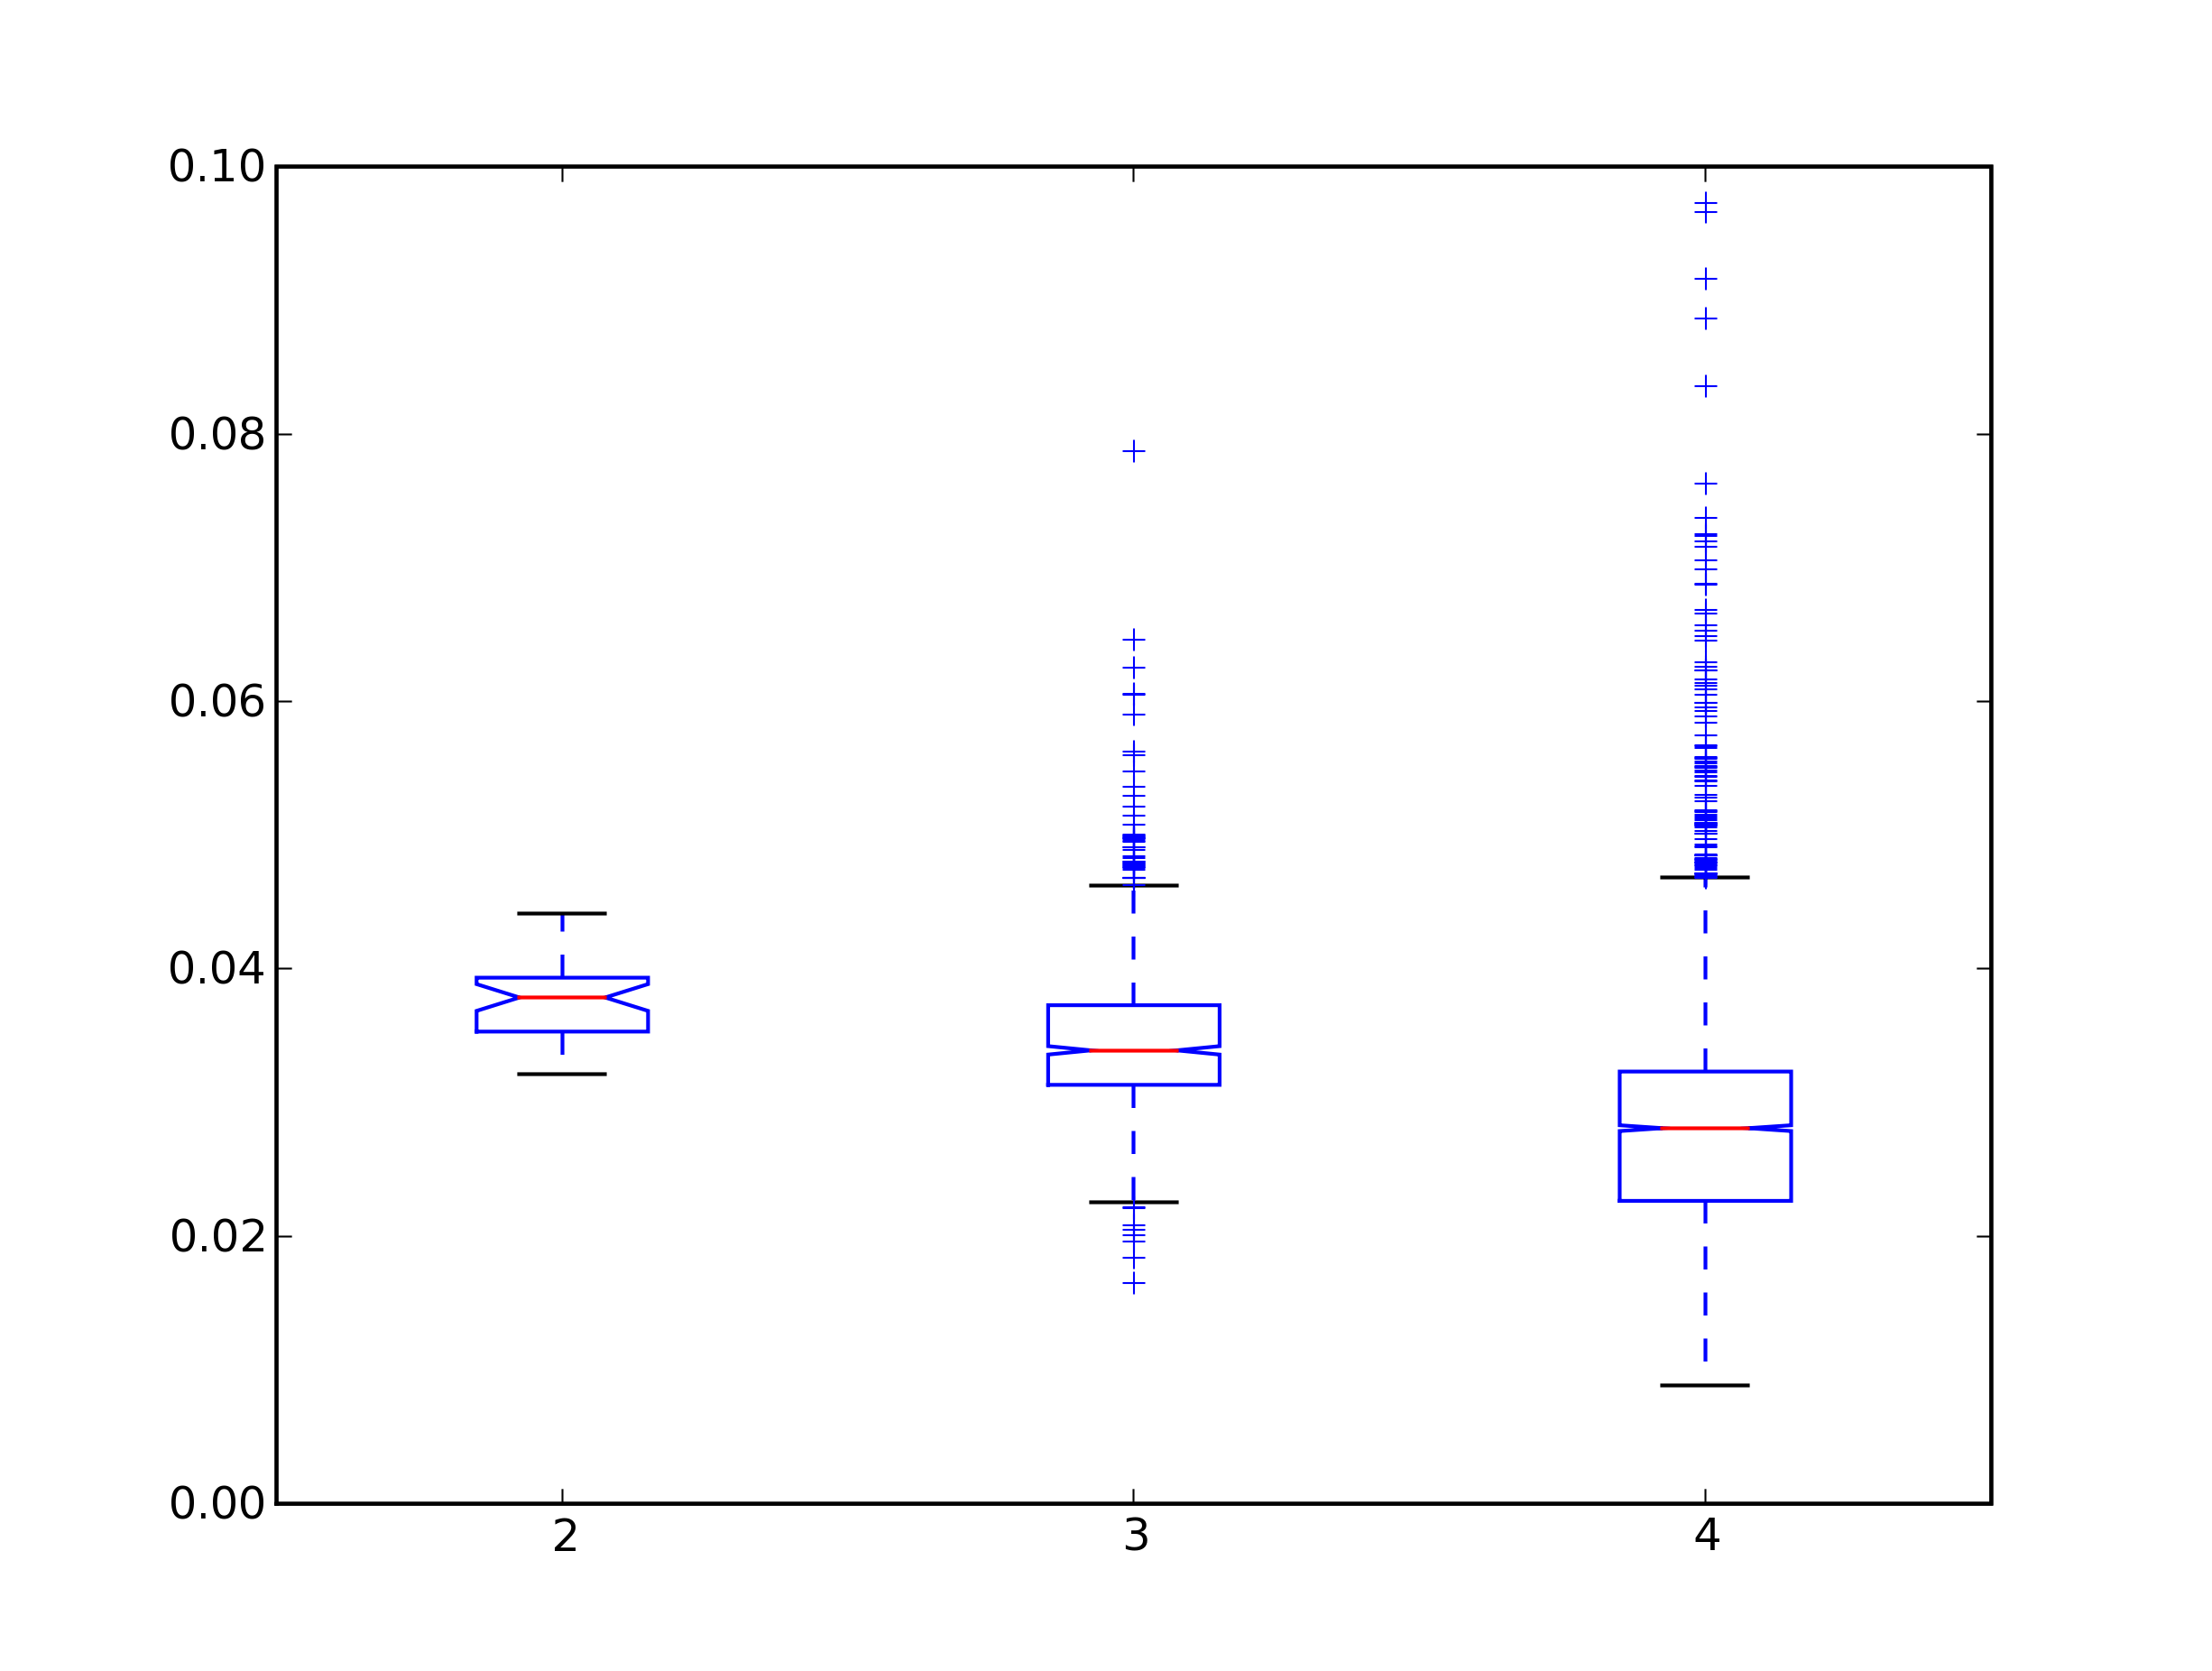
\includegraphics[width=.45\linewidth]{rook_iv_box.png}
}
\subfigure[Hexagonal Topology]{
  \label{boxplot:hex}
  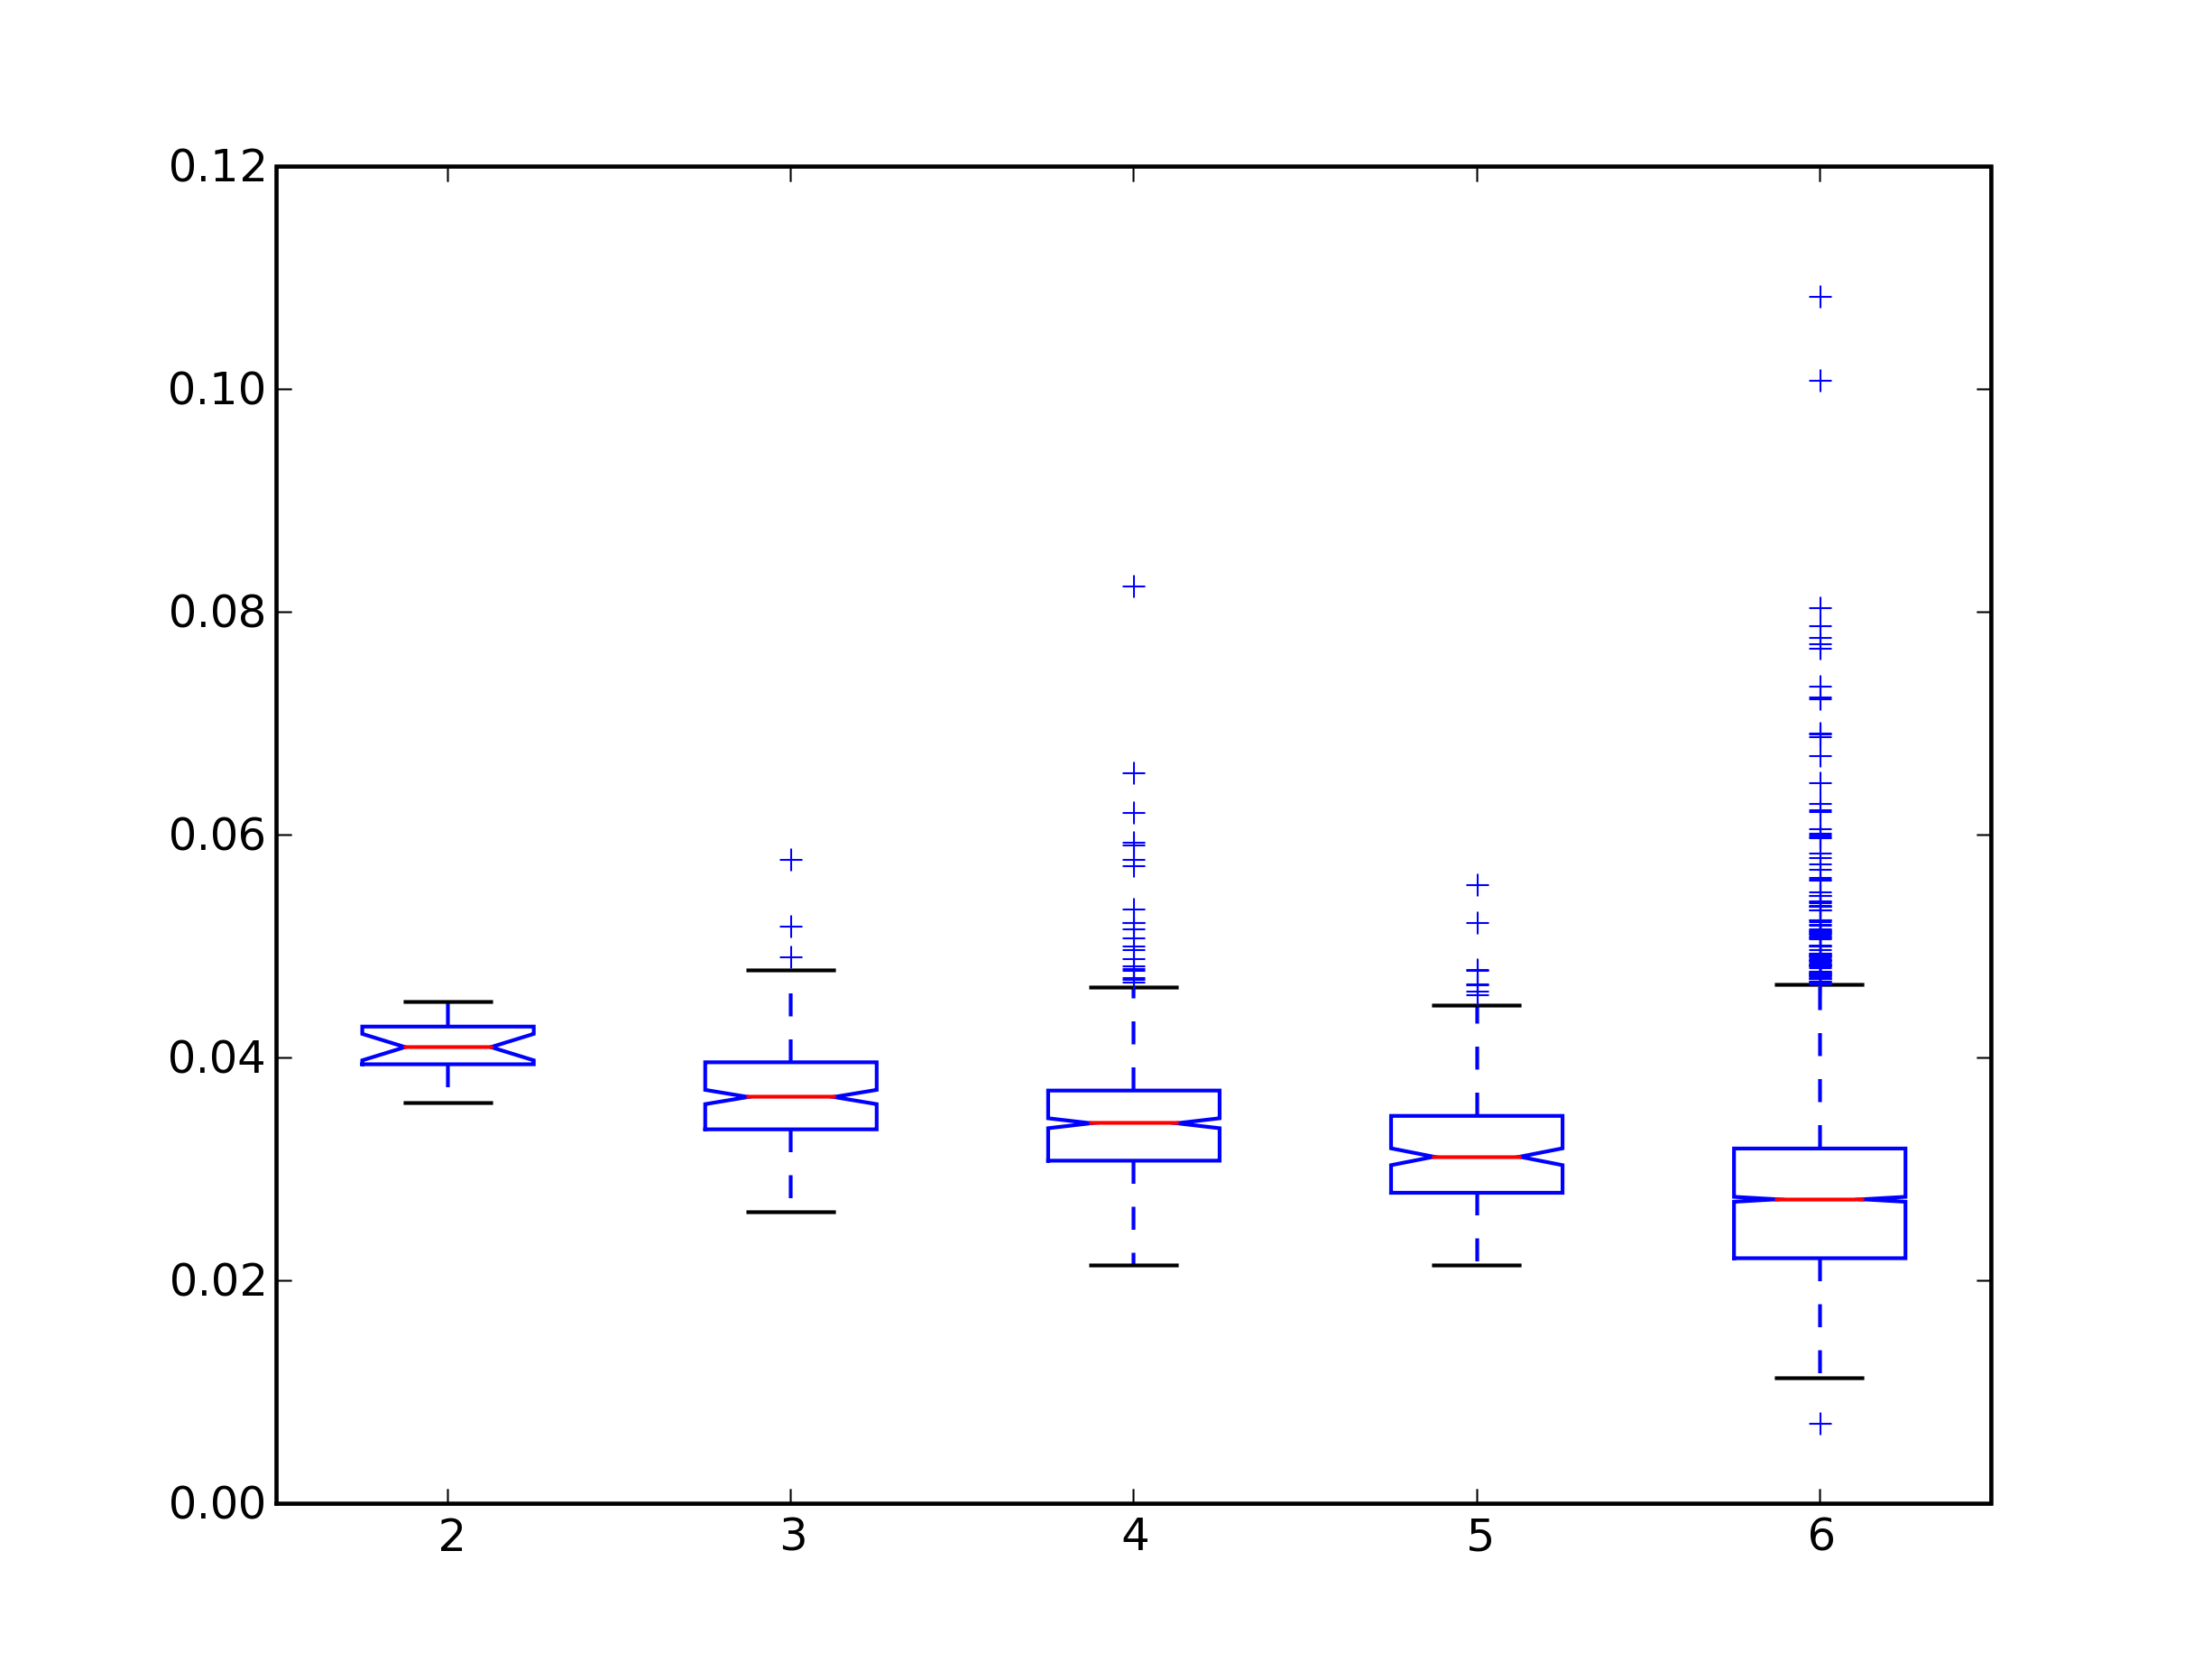
\includegraphics[width=.45\linewidth]{hex_iv_box.png}
}
\subfigure[Spherical Topology]{
  \label{boxplot:graph}
  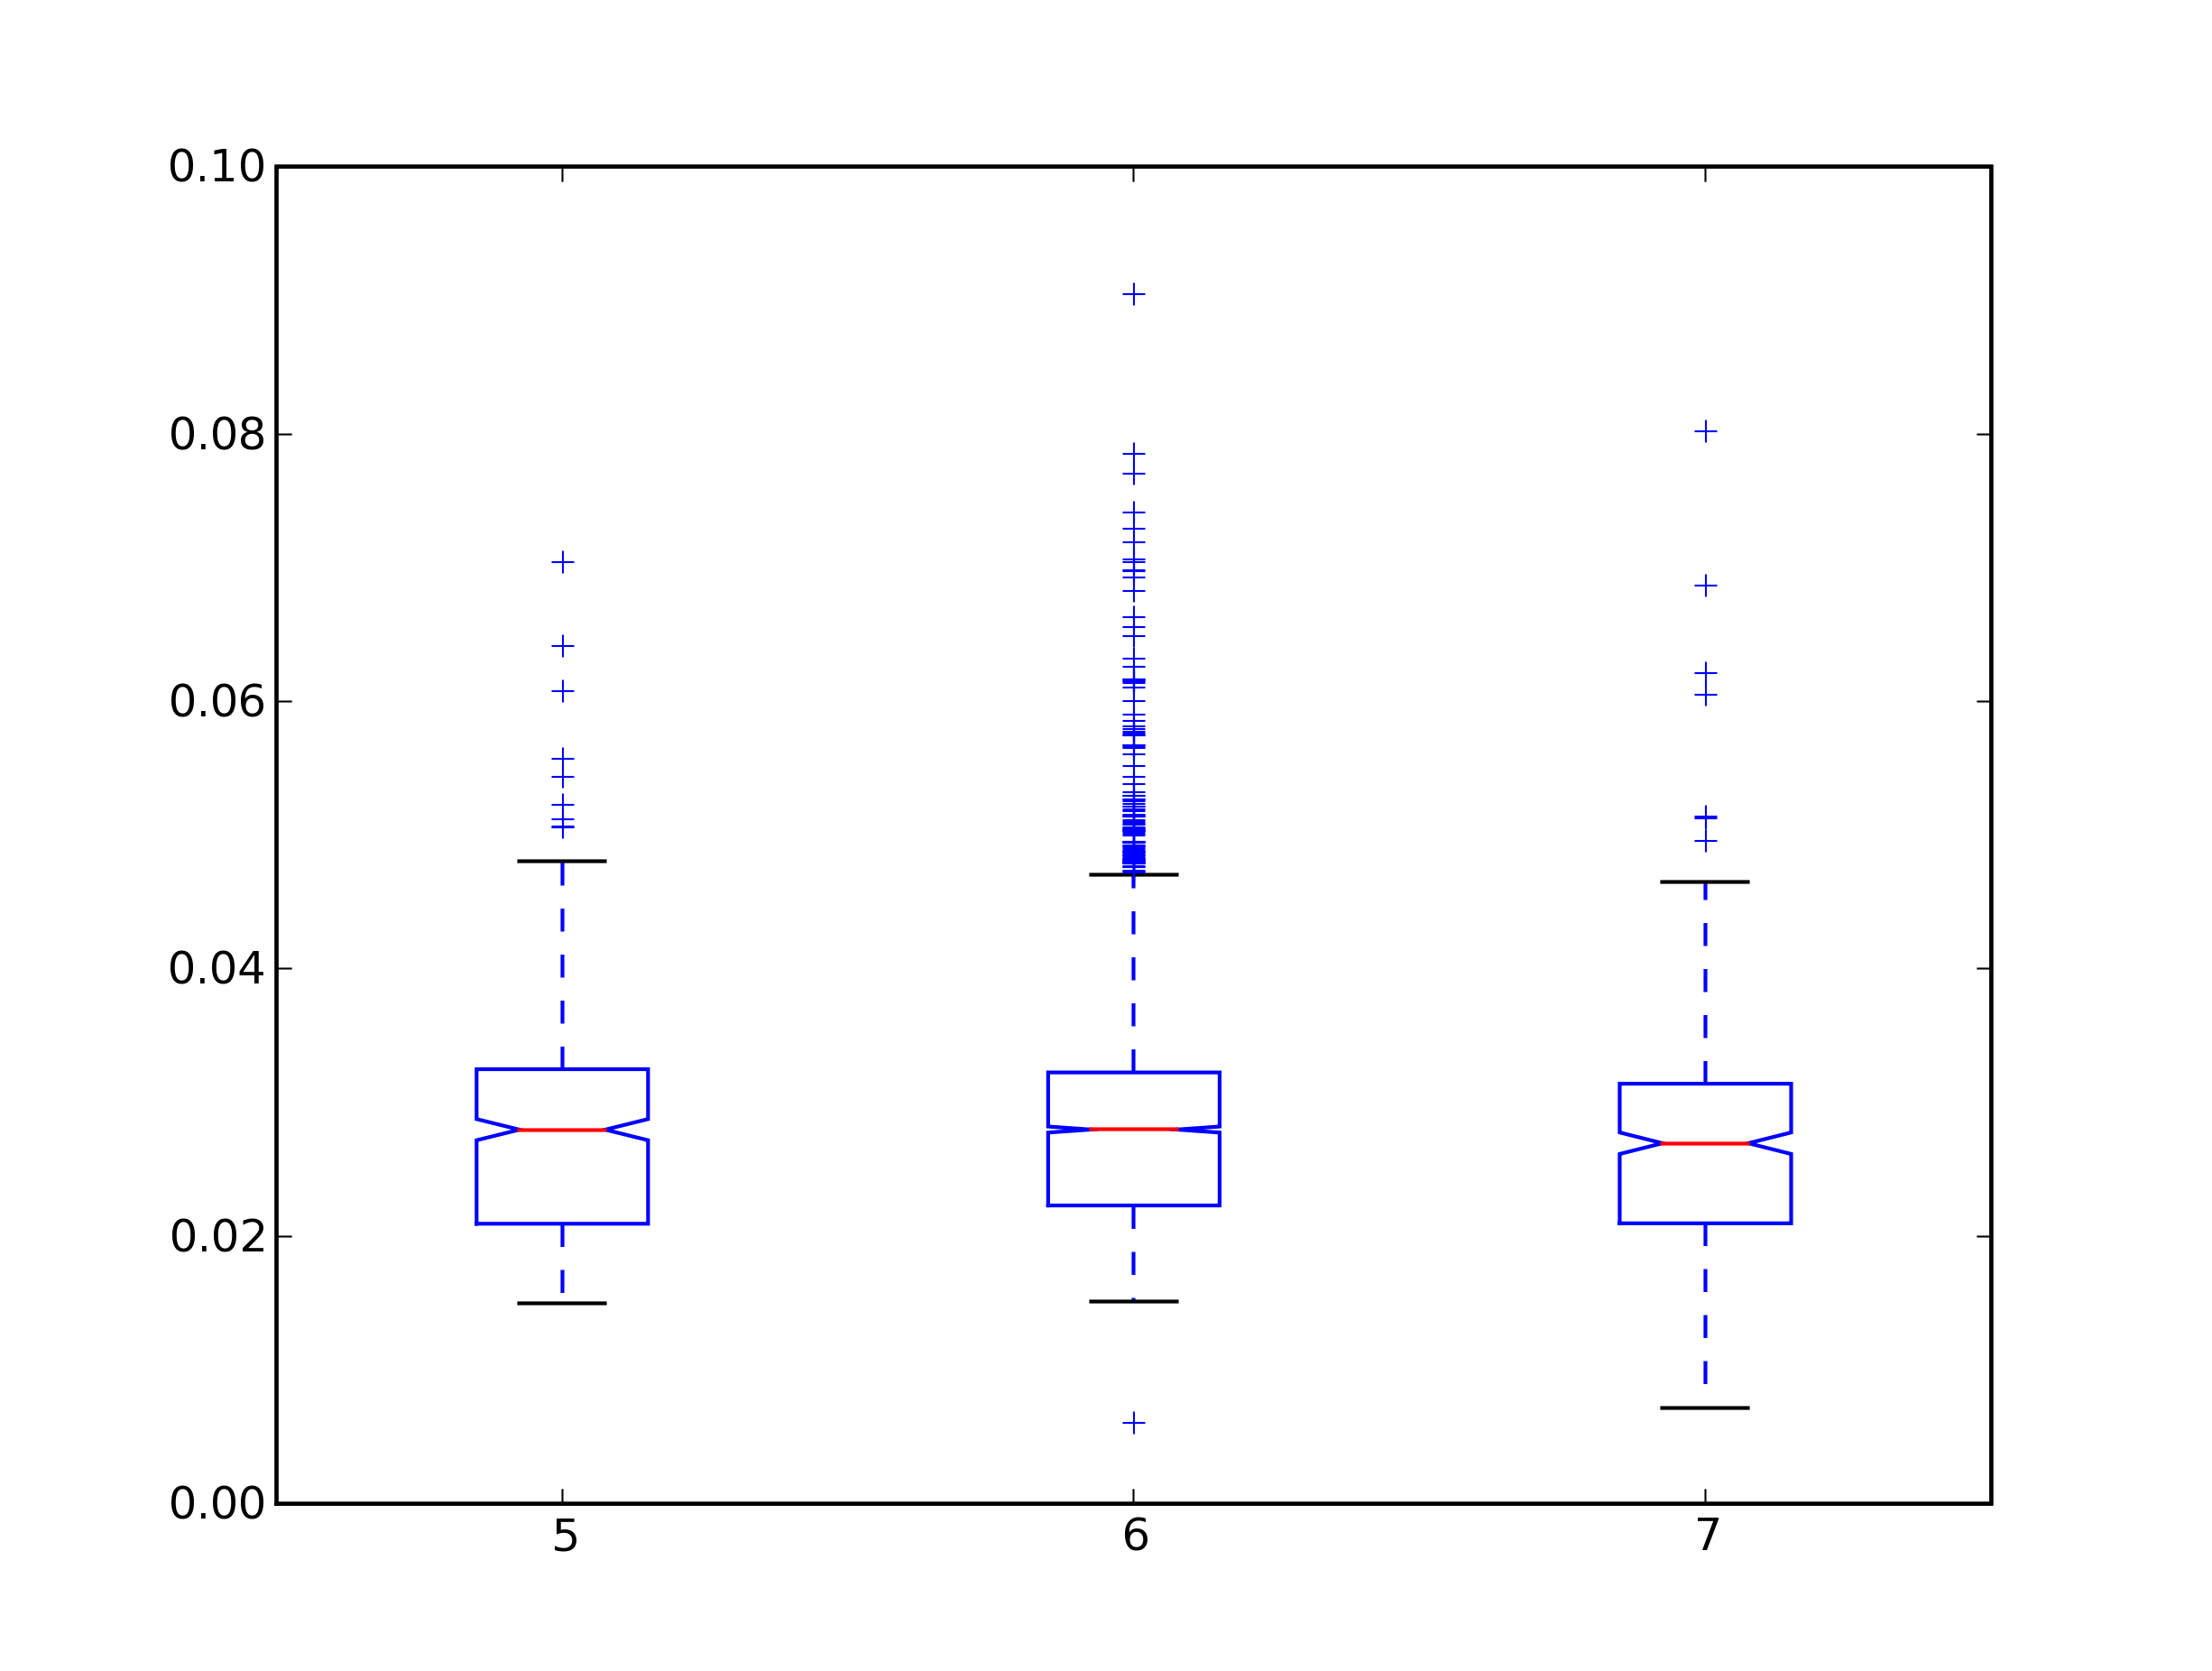
\includegraphics[width=.45\linewidth]{graph_iv_box.png}
}
\subfigure[Geodesic Sphere Topology]{
  \label{boxplot:geodesic}
  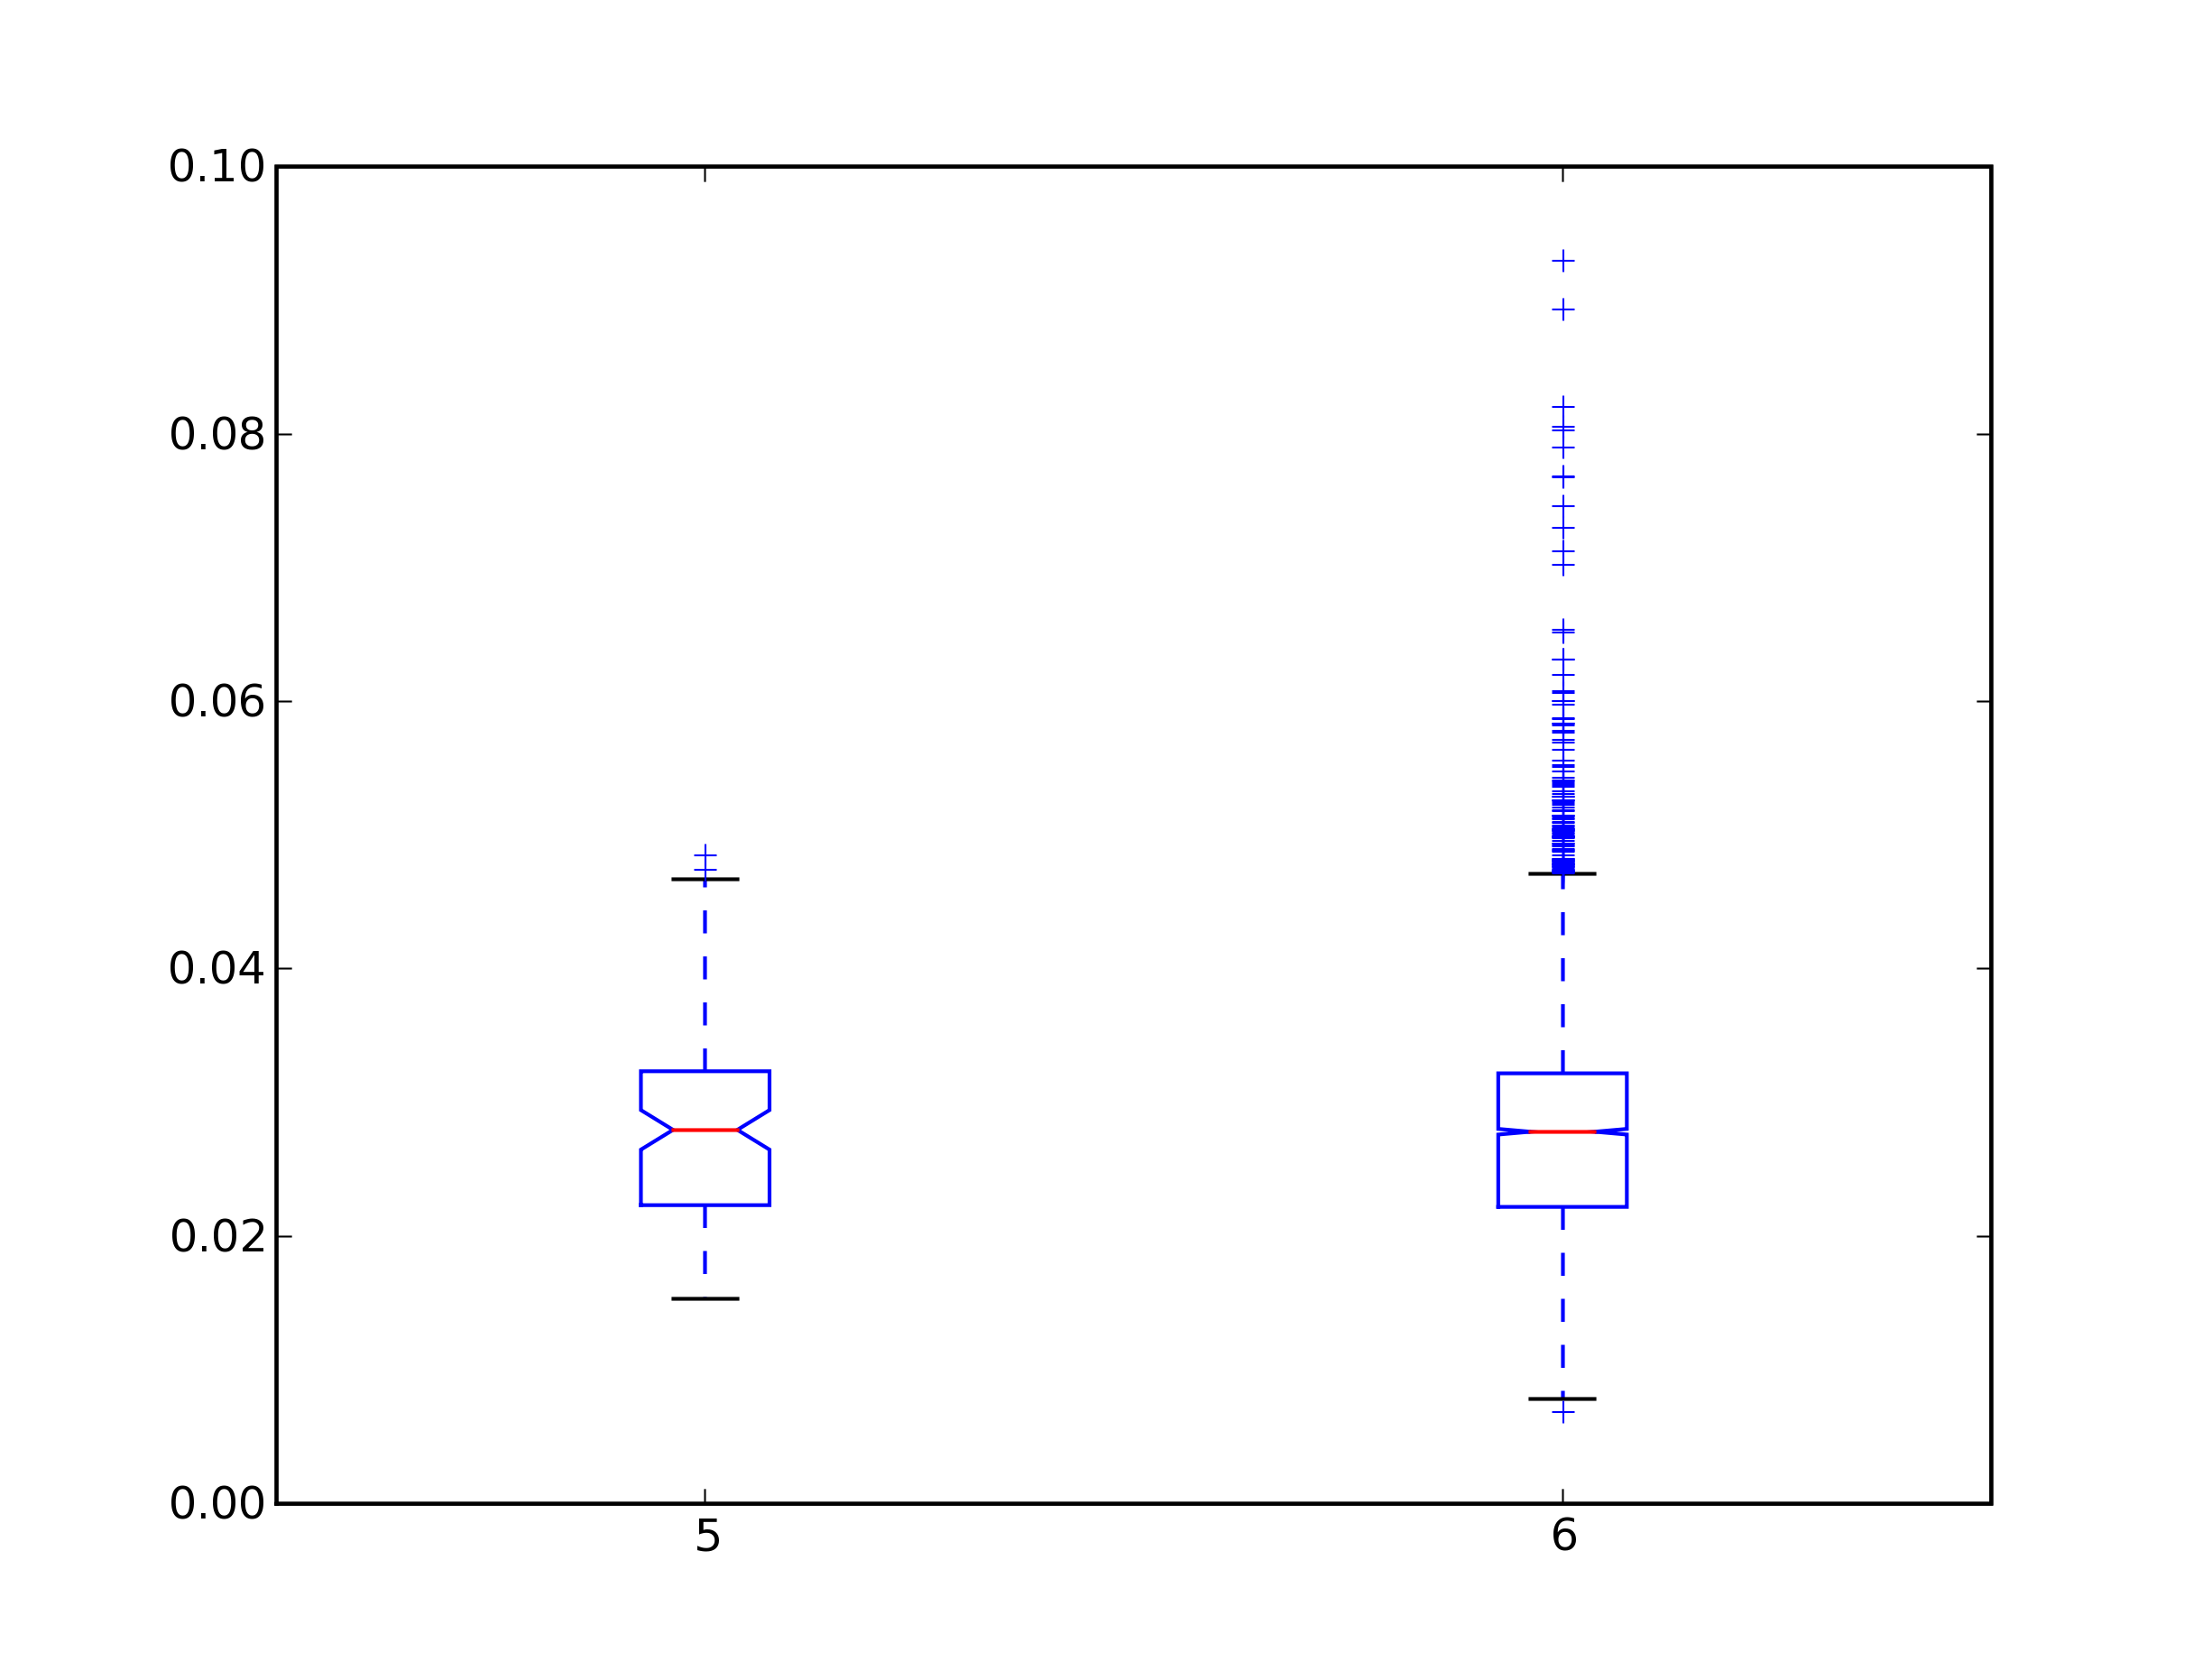
\includegraphics[width=.45\linewidth]{geodesic_iv_box.png}
}
\caption{Box-and-whisker diagrams representing samples derived from forty
trained SOMs.  The samples within each topology were created by grouping the
internal variance of each neuron of a given degree size. The diagrams how the
centrality and dispersion of each sample.}
\label{boxplot}
\end{figure}

%I suspect a better measure would be to use the minimum number of steps for a
%given nueron to reach every other neuron on the network.  This would vary
%significantly on the rook and hexagon topolgoies, but not very much in the
%spherical topologies.

%\begin{landscape}
\begin{table}
\centering
\scriptsize
\begin{minipage}{\textwidth}
\caption{Size, mean and variance of each sample}
\label{meanvar1}
\begin{tabular}{|c||cc|cc|cc|cc|}
\hline
\textbf{Degree} & \multicolumn{2}{c|}{\textbf{Geodesic}} &
\multicolumn{2}{c|}{\textbf{Spherical}} &
\multicolumn{2}{c|}{\textbf{Hexagonal}} &
\multicolumn{2}{c|}{\textbf{Rectangular}} \\
\hline
& N & Mean (Var) & N & Mean (Var) & N & Mean (Var) & N & Mean (Var) \\
\hline
2&&&&& 20& 0.0409 (5.66E-06)& 40& 0.0378 (7.59E-06)\\ 
3&&&&& 218& 0.0371 (2.18E-05)& 880& 0.0348 (3.59E-05)\\ 
4&&&&& 489& 0.0347 (4.05E-05)& 4926& 0.0284 (6.28E-05)\\ 
5& 113& 0.0283 (5.28E-05)& 526& 0.0279 (6.43E-05)& 206& 0.0319 (3.50E-05)&&\\ 
6& 5598& 0.0281 (6.05E-05)& 4758& 0.0282 (6.05E-05)& 4954& 0.0278
(6.09E-05)&&\\ 
7&&& 417& 0.0273 (6.65E-05)&&&&\\ 
\hline
\end{tabular} \end{minipage} \end{table}
%\end{landscape}



%\subsection{Restate the Questions}
%\textbf{Objective}, Compare the internal variance of observations captured by a given
%neuron to that neuron's first-order neighborhood size.
%\textbf{Question}, Does the internal variance of a neuron decrease as its first-order
%neighborhood size, or degree, increases?


\begin{table}
\begin{minipage}{\textwidth}
\caption{Results of Difference of Mean Testing Within Each Topology}
\label{rlt}


  \subtable[Rectangular Topology]{
    \label{rlt:rook}
    \begin{tabular}{|c||c|c|c|}
    \hline
    Degree&2&3&4\\\hline
    \hline
    2 & (0.000008) & \textbf{0.002700} & \textbf{0.000100}\\\hline
    3 & 0.002969 & (0.000036) & \textbf{0.000100}\\\hline
    4 & 0.009364 & 0.006396 & (0.000063)\\\hline
    \end{tabular}
  }

  \subtable[Hexagonal Topology]{
    \label{rlt:hex}
    \begin{tabular}{|c||c|c|c|c|c|}
    \hline
    Degree&2&3&4&5&6\\ \hline
    \hline
    2 & (0.000006) & \textbf{0.000800} & \textbf{0.000200} & \textbf{0.000100} & \textbf{0.000100}\\\hline
    3 & 0.003810 & (0.000022) & \textbf{0.000100} & \textbf{0.000100} & \textbf{0.000100}\\\hline
    4 & 0.006253 & 0.002443 & (0.000040) & \textbf{0.000100} & \textbf{0.000100}\\\hline
    5 & 0.009008 & 0.005197 & 0.002755 & (0.000035) & \textbf{0.000100}\\\hline
    6 & 0.013067 & 0.009257 & 0.006814 & 0.004059 & (0.000061)\\\hline
    \end{tabular}
  }

  \subtable[Spherical Topology]{
    \label{rlt:graph}
    \begin{tabular}{|c||c|c|c|}
    \hline	
    Degree&5&6&7\\ \hline
    \hline
    5 & (0.000064) & 0.485500 & 0.197400\\\hline
    6 & 0.000250 & (0.000060) & \textbf{0.020000}\\\hline
    7 & 0.000674 & 0.000924 & (0.000067)\\\hline
    \end{tabular}
  }

  \subtable[Geodesic Topology]{
    \label{rlt:geodesic}
    \begin{tabular}{|c||c|c|}
    \hline
    Degree&5&6\\ \hline
    \hline
    5 & (0.000053) & 0.783900\\\hline
    6 & 0.000203 & (0.000060)\\\hline
    \end{tabular}
  }
\end{minipage}\end{table}

\section{Internal variance vs. centrality}
\label{rdq2}
The degree of a node on a network is a measure of its centrality, or
importance. Nodes with more connections are thought to be more central to
the network and have a larger influence than nodes with fewer connections. As an
artifact of the training process observations that are more average than
others tend to be centralized.  The observations that surround them tend to be
more extreme.  If you refer back to figure \ref{figure1}, you'll notice that
observations with smaller symbols are closer to the mean of all the
observations and that these observations have been centralized in the network.
Using the degree as a measure of centrality does not capture this picture
well, as neurons near the edge can still have a large degree.  A way to
capture this effect would be to look at closeness centrality, which is the
inverse of the average distance of a neuron to every other neuron on the
network.

Above we saw that changes in a neuron's degree was related to changes in
internal variance in topologies with edges, but not in the two sphere-based
topologies. The next step is to see if internal variance changes between
topologies.  To do this we will first order our topologies by a summary
measure of the network centrality.  For this diagnostic we use the average
closeness centrality for each topology as the summary measure.  The summary
measure and the sorting of our topologies is shown in table \ref{vardeg}.

\begin{table}
\centering
\begin{minipage}{\textwidth}
\caption{Measure of Topological Regularity and Sample Mean and Variance}
\label{vardeg}
\begin{tabular}{|c||c|c|c|}
\hline
Topology & Closeness Centrality & Mean & Variance\\
\hline
Rectangular & 0.0603 & 0.0294 &0.0001\\
Hexagonal & 0.0739 & 0.0289 &0.0001\\
Geodesic & 0.0890 & 0.0281 &0.0001\\
Spherical & 0.0906 & 0.0281 &0.0001\\
\hline
\end{tabular}
\end{minipage}
\end{table}

In this diagnostic we group the samples from the previous section by topology.
This results in one sample for each of the four topologies.  We test for a
difference in mean and variance between each sample using the same method of
random labeling that was applied in the previous diagnostic.  No significant
differences were found in the variances; the difference in means are presented
in table \ref{rlt:all}.  It was expected that the mean and variance of the
samples would decrease for the more regular topologies.  These results
generally support this hypothesis. We see that the rectangular topology has
the highest mean internal variance and is the least regular as measured by
closeness centrality. The geodesic and spherical topologies are the most
regular and have the lowest internal variance. These two groups display very
similar measures of closeness centrality and show no significant difference in
mean internal variance.  This suggests that even though the spherical topology
is more irregular than the geodesic topology, similar levels of quality may be
achieved.


\begin{table}
  \begin{minipage}{\textwidth}
  \caption{Results of Difference of Mean Testing Across Topologies}
  \label{rlt:all}
  \begin{tabular}{|c||c|c|c|c|}
  \hline
  \textbf{Topology}&Rectangular	&Hexagonal &Geodesic &Spherical\\\hline
  \hline
   Rectangular & (0.000064) & \textbf{0.001000} & \textbf{0.000100} & \textbf{0.000100}\\\hline
   Hexagonal & -0.000479 & (0.000064) & \textbf{0.000100} & \textbf{0.000100}\\\hline
   Geodesic & -0.001329 & -0.000850 & (0.000060) & 0.505600\\\hline
   Spherical & -0.001328 & -0.000849 & 0.000001 & (0.000061)\\\hline

  \end{tabular}
  \end{minipage}
\end{table}



\section{Visualization of internal variance}
\label{rdq3}
In order to address our research questions we first created ten synthetic
datasets.  Each was created by sampling from the same data generating process
that was provided by \cite{wu2006}.  We used these datasets to train ten
SOMs for each of our topologies.  The purpose of training ten SOMs was to
produce large enough samples sizes for the difference of means and variance
testing that was necessary to formally evaluate the results of our first two
research questions.  In this section we quickly verify that combining those
simulations was appropriate by visualizing the similarities between them.
In the remainder of this section we focus our efforts on comparing across
topologies.  Since we have seen that little variation exists between the ten
simulations we pick the first of those simulations for each topology and
explore them in more depth.

We look at what information can be gained from visualizing the SOM and its
internal variance. In order to create these visualizations we used
off-the-shelf GIS packages, namely ESRI's ArcGIS.  There are a number of
challenges which had to be overcome. To visualize the rectangular and
hexagonal topologies we simply created polygons centered over each neuron.
However, the spherical and geodesic topologies were slightly more complicated.
To create the polygons for these topologies we must first computed the Voronoi
diagram on the surface of the sphere.  This is done using STRIPACK, a software
program created by \cite{Ranka97}.  Further, ArcGIS and other common GIS
packages assume Cartesian distances and thus can not handle polygons that
cross the $180^{th}$ meridian.  To accommodate this we split each polygon at
the $180^{th}$ meridian and redrew it as two parts.  

As expected, figure \ref{ten} reveals little variation 
between simulations of a given topology.  This homogeneity demonstrates that
our ten synthetic datasets adequately increase our sample size without introducing bias.  
Because of the apparent homogeneity between the simulations \emph{within} a
given topology, we move on to compare the first simulation \emph{across} topologies.  
Our synthetic training data consisted of seven clusters located in three
dimensional space. We examine how the SOM treats the original data through a
series of visualizations.  The component planes in figure \ref{cplanes} show
how the SOM represents each dimension of the training data.  The variations we
see in the placement of high and low values, between topologies, is caused by
the random initialization of the SOM.  However, the relationships between the
dimensions remain constant across topologies.  Figure \ref{cluster} shows how
the SOM detected the clustering of the input data.  We calculated the cluster
to which a neuron belongs by looking at the observations mapped to it.
Knowing which cluster each observation belongs to allows to see where the
clusters are being mapped on the trained SOM. For a given neuron we classify
it by the most frequent cluster it captured.  It is interesting to note that
the edges of the cluster exhibit high internal variance.

This is somewhat intuitive, as our clusters are normally distributed, the
majority of our observations will fall well within the regions observed in
figure \ref{cluster}. Each cluster's outliers will be pushed toward the
``edges'' of these regions. In the hexagonal and rectangular topologies
some of these cluster regions share and edge with the topology itself.  This
allows their outlying observation to interact less with the interior neurons.
In the spherical and geodesic topologies outliers pushed toward the edge of
their cluster's region on the map are force to interact with other neurons.

%The particulars of synthetic dataset in combination with these visualizations
%may raise questions about the suitability of sphere based SOMs in certain
%applications.  Specifically, extreme observations in our dataset (those
%furthest from the origin), may be well represented on the edge of the flat
%topologies where there are furthest away from their counter parts in the other
%extreme.  This may hold true in the spherical topologies as well if these
%extreme observations are antipodal, in fact it might be even better
%represented.


 , at these locations they could be pushed 

\begin{figure}
\centering
\begin{minipage}{\textwidth}
\subfigure[Rectangular Topology]{
  \label{ten:rook}
  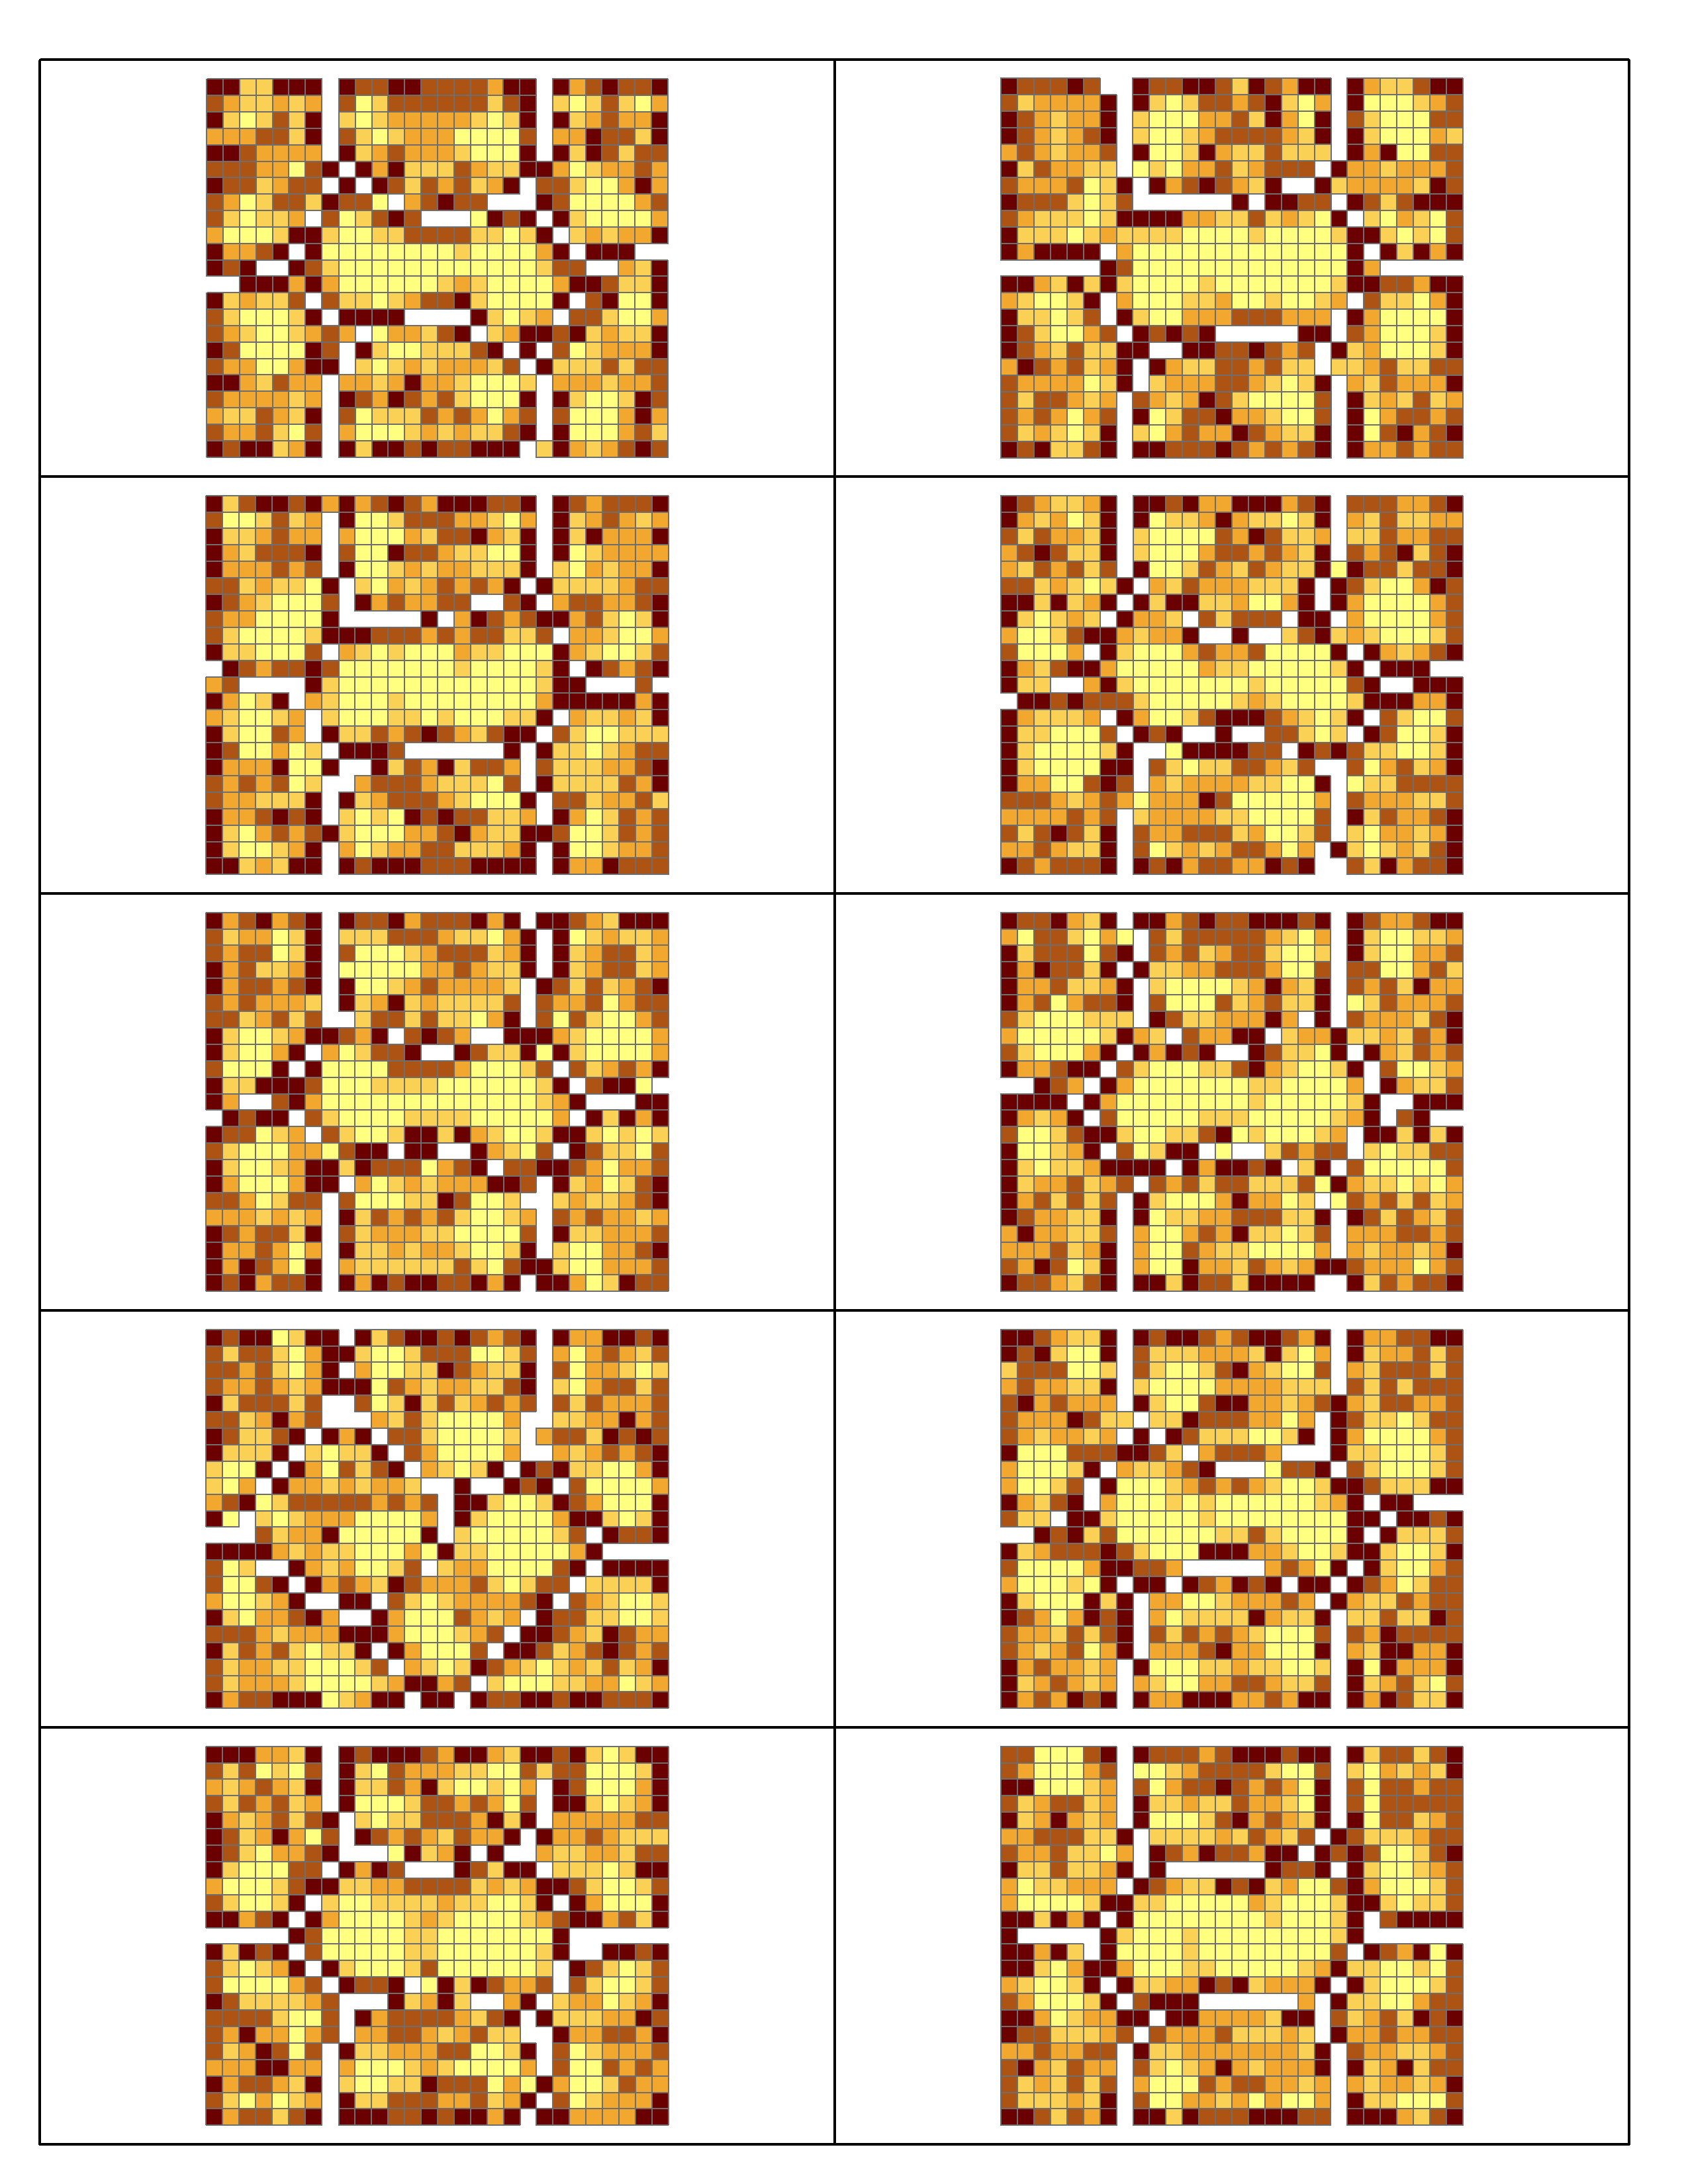
\includegraphics[width=0.5\linewidth]{rook_thesis_7c.png}
}
\subfigure[Hexagonal Topology]{
  \label{ten:hex}
  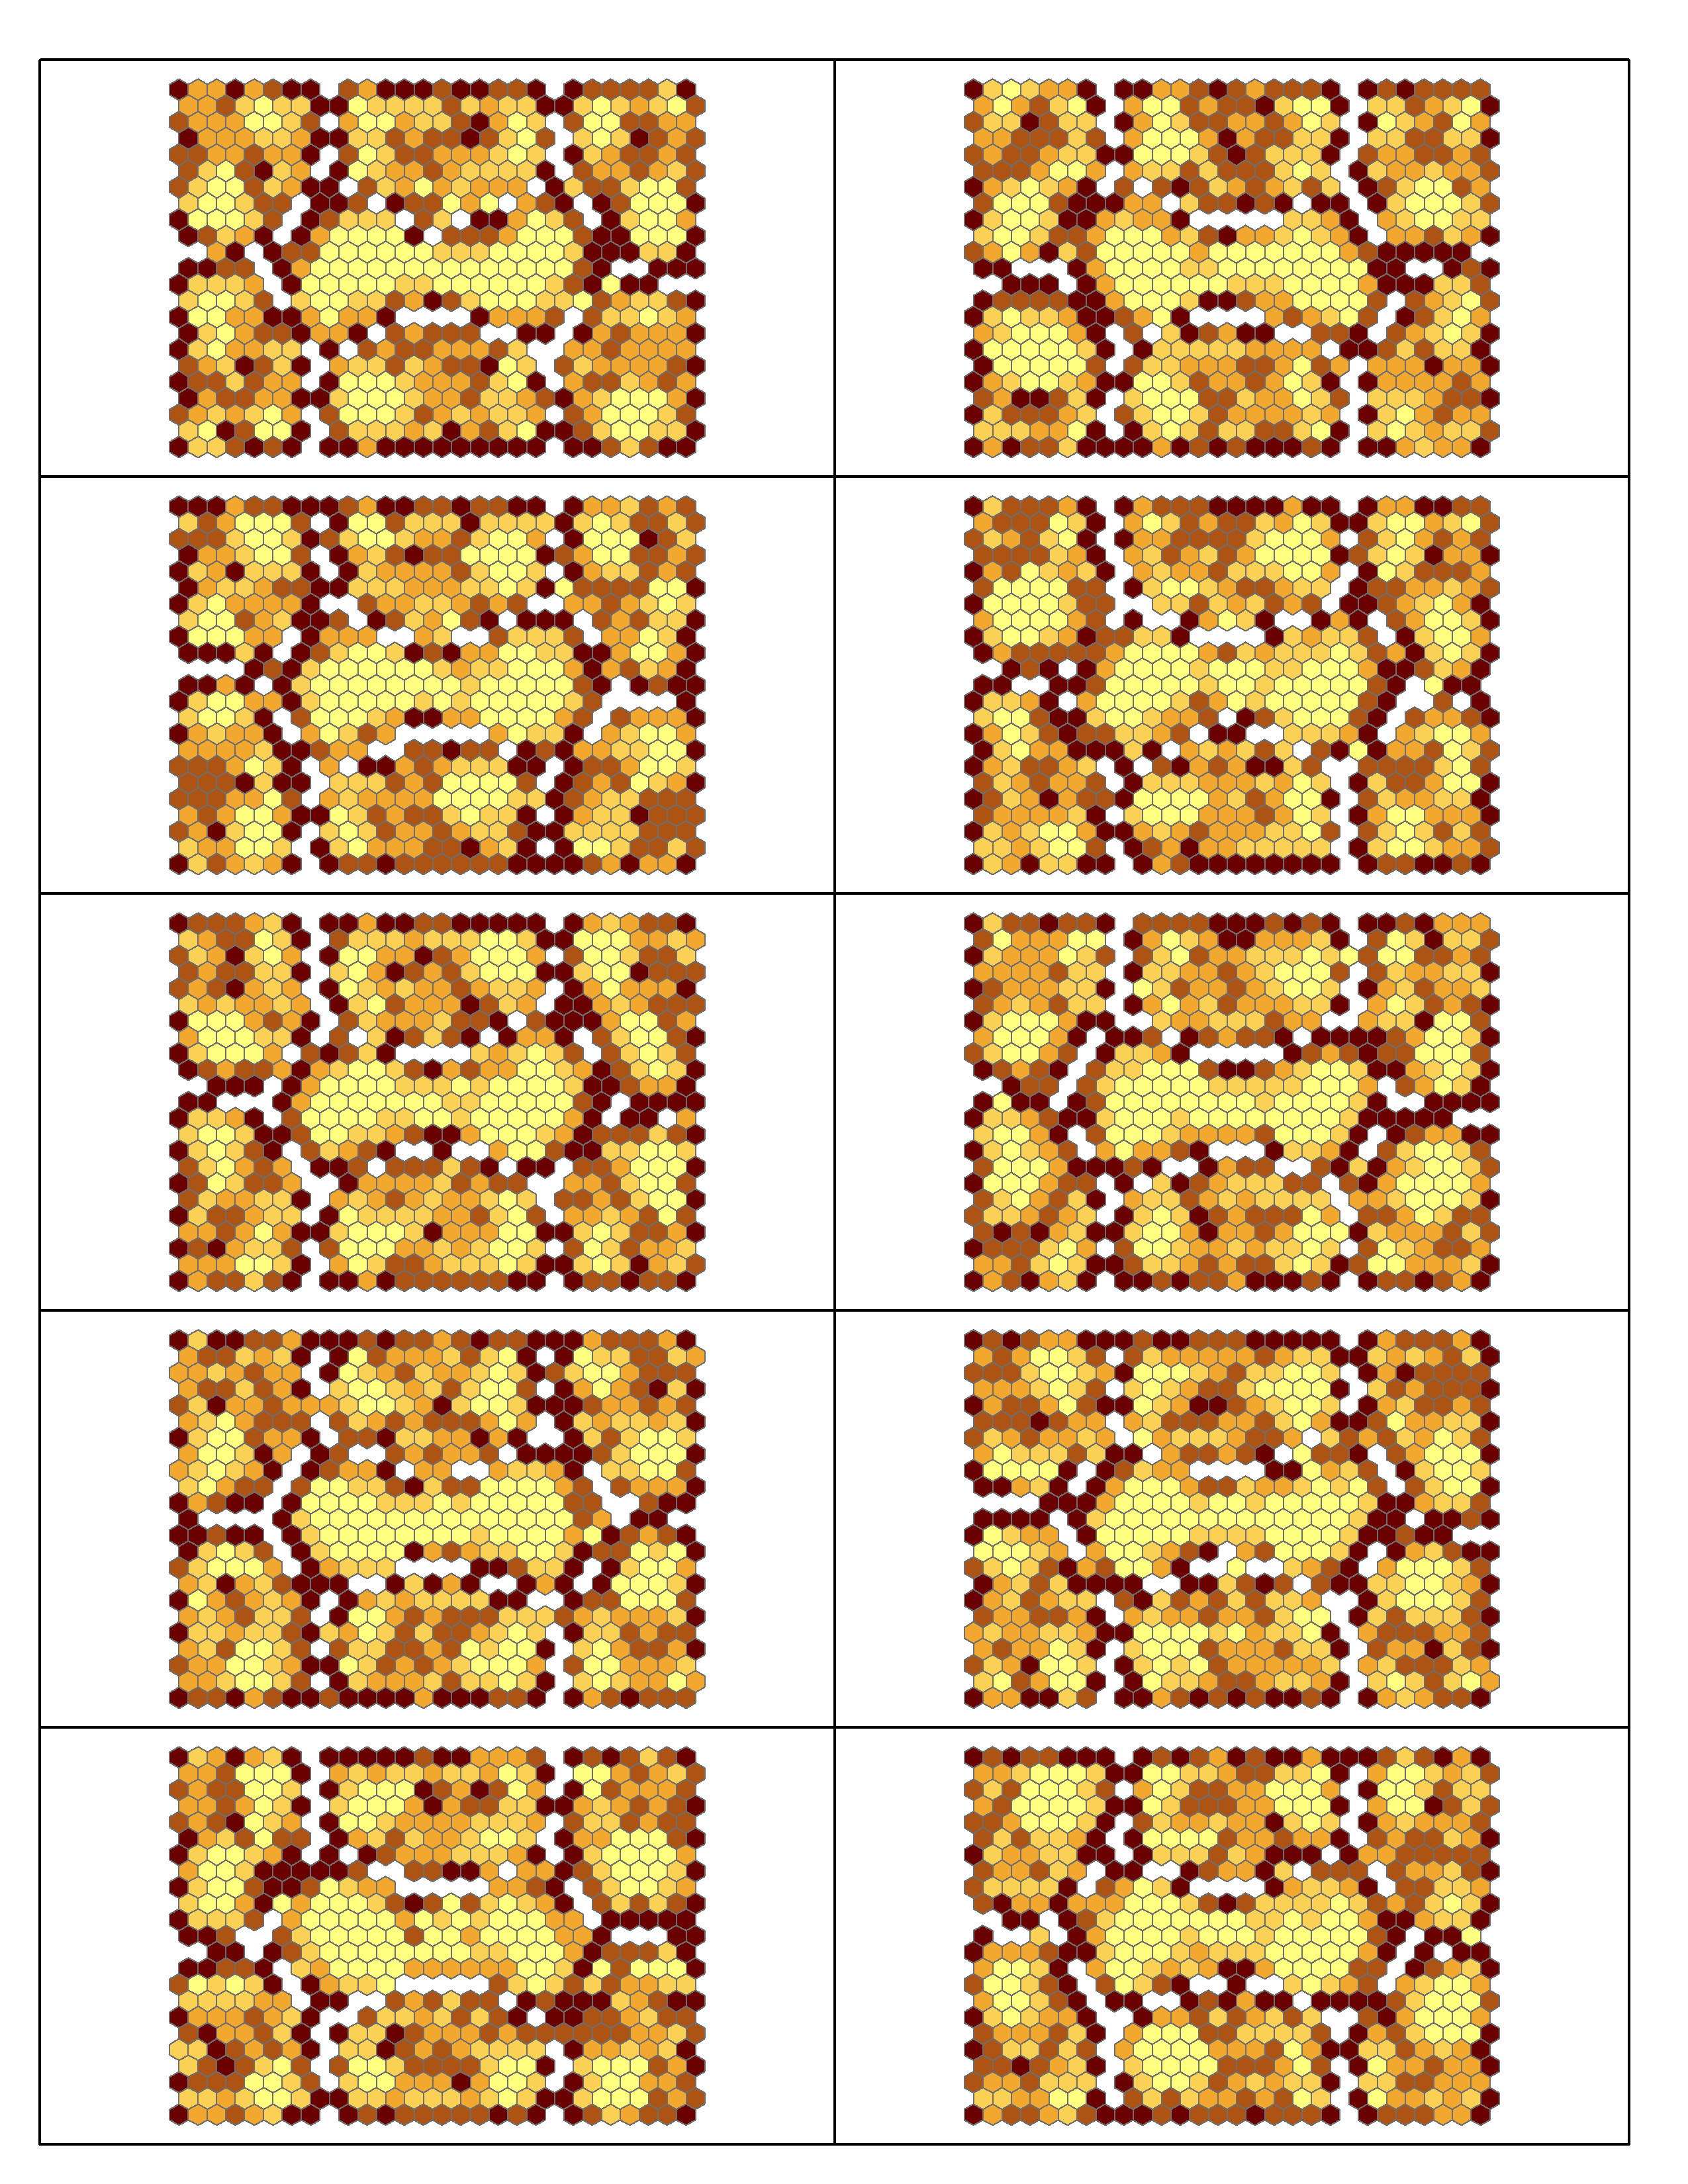
\includegraphics[width=0.5\linewidth]{hex_thesis_7c.png}
}
\subfigure[Spherical Topology]{
  \label{ten:graph}
  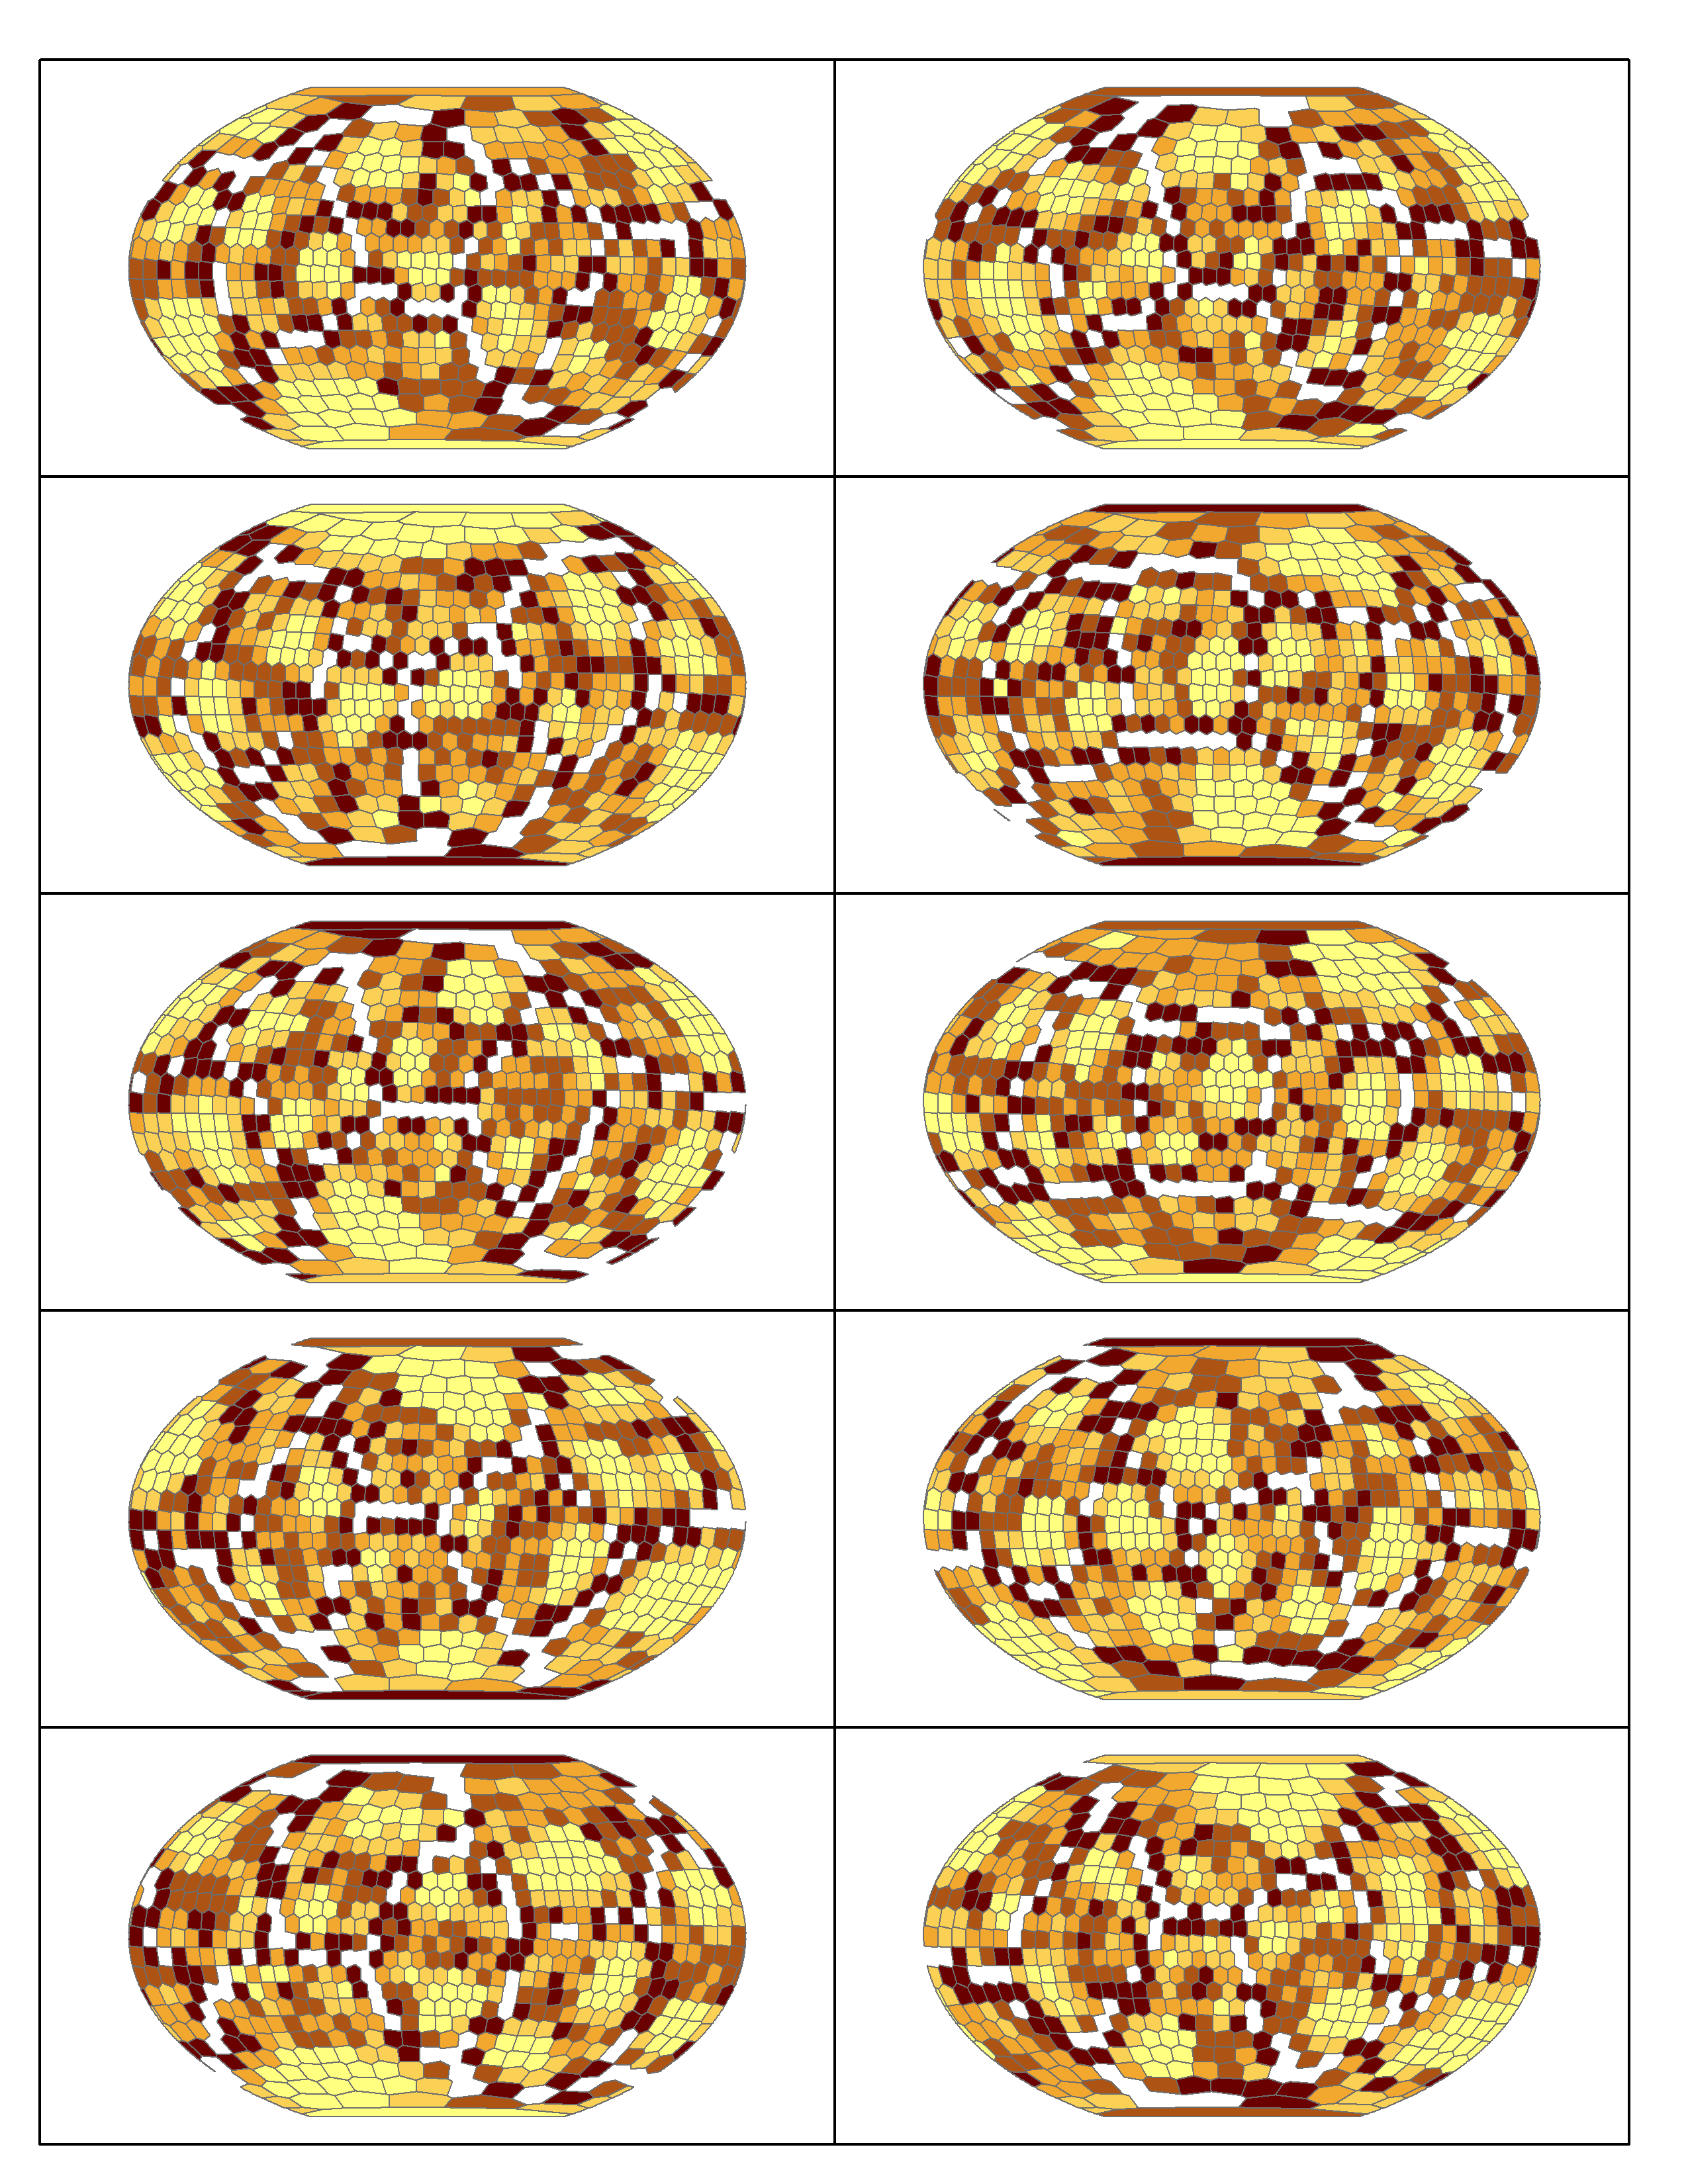
\includegraphics[width=0.5\linewidth]{sphere_thesis_7c.png}
}
\subfigure[Geodesic Sphere Topology]{
  \label{ten:geodesic}
  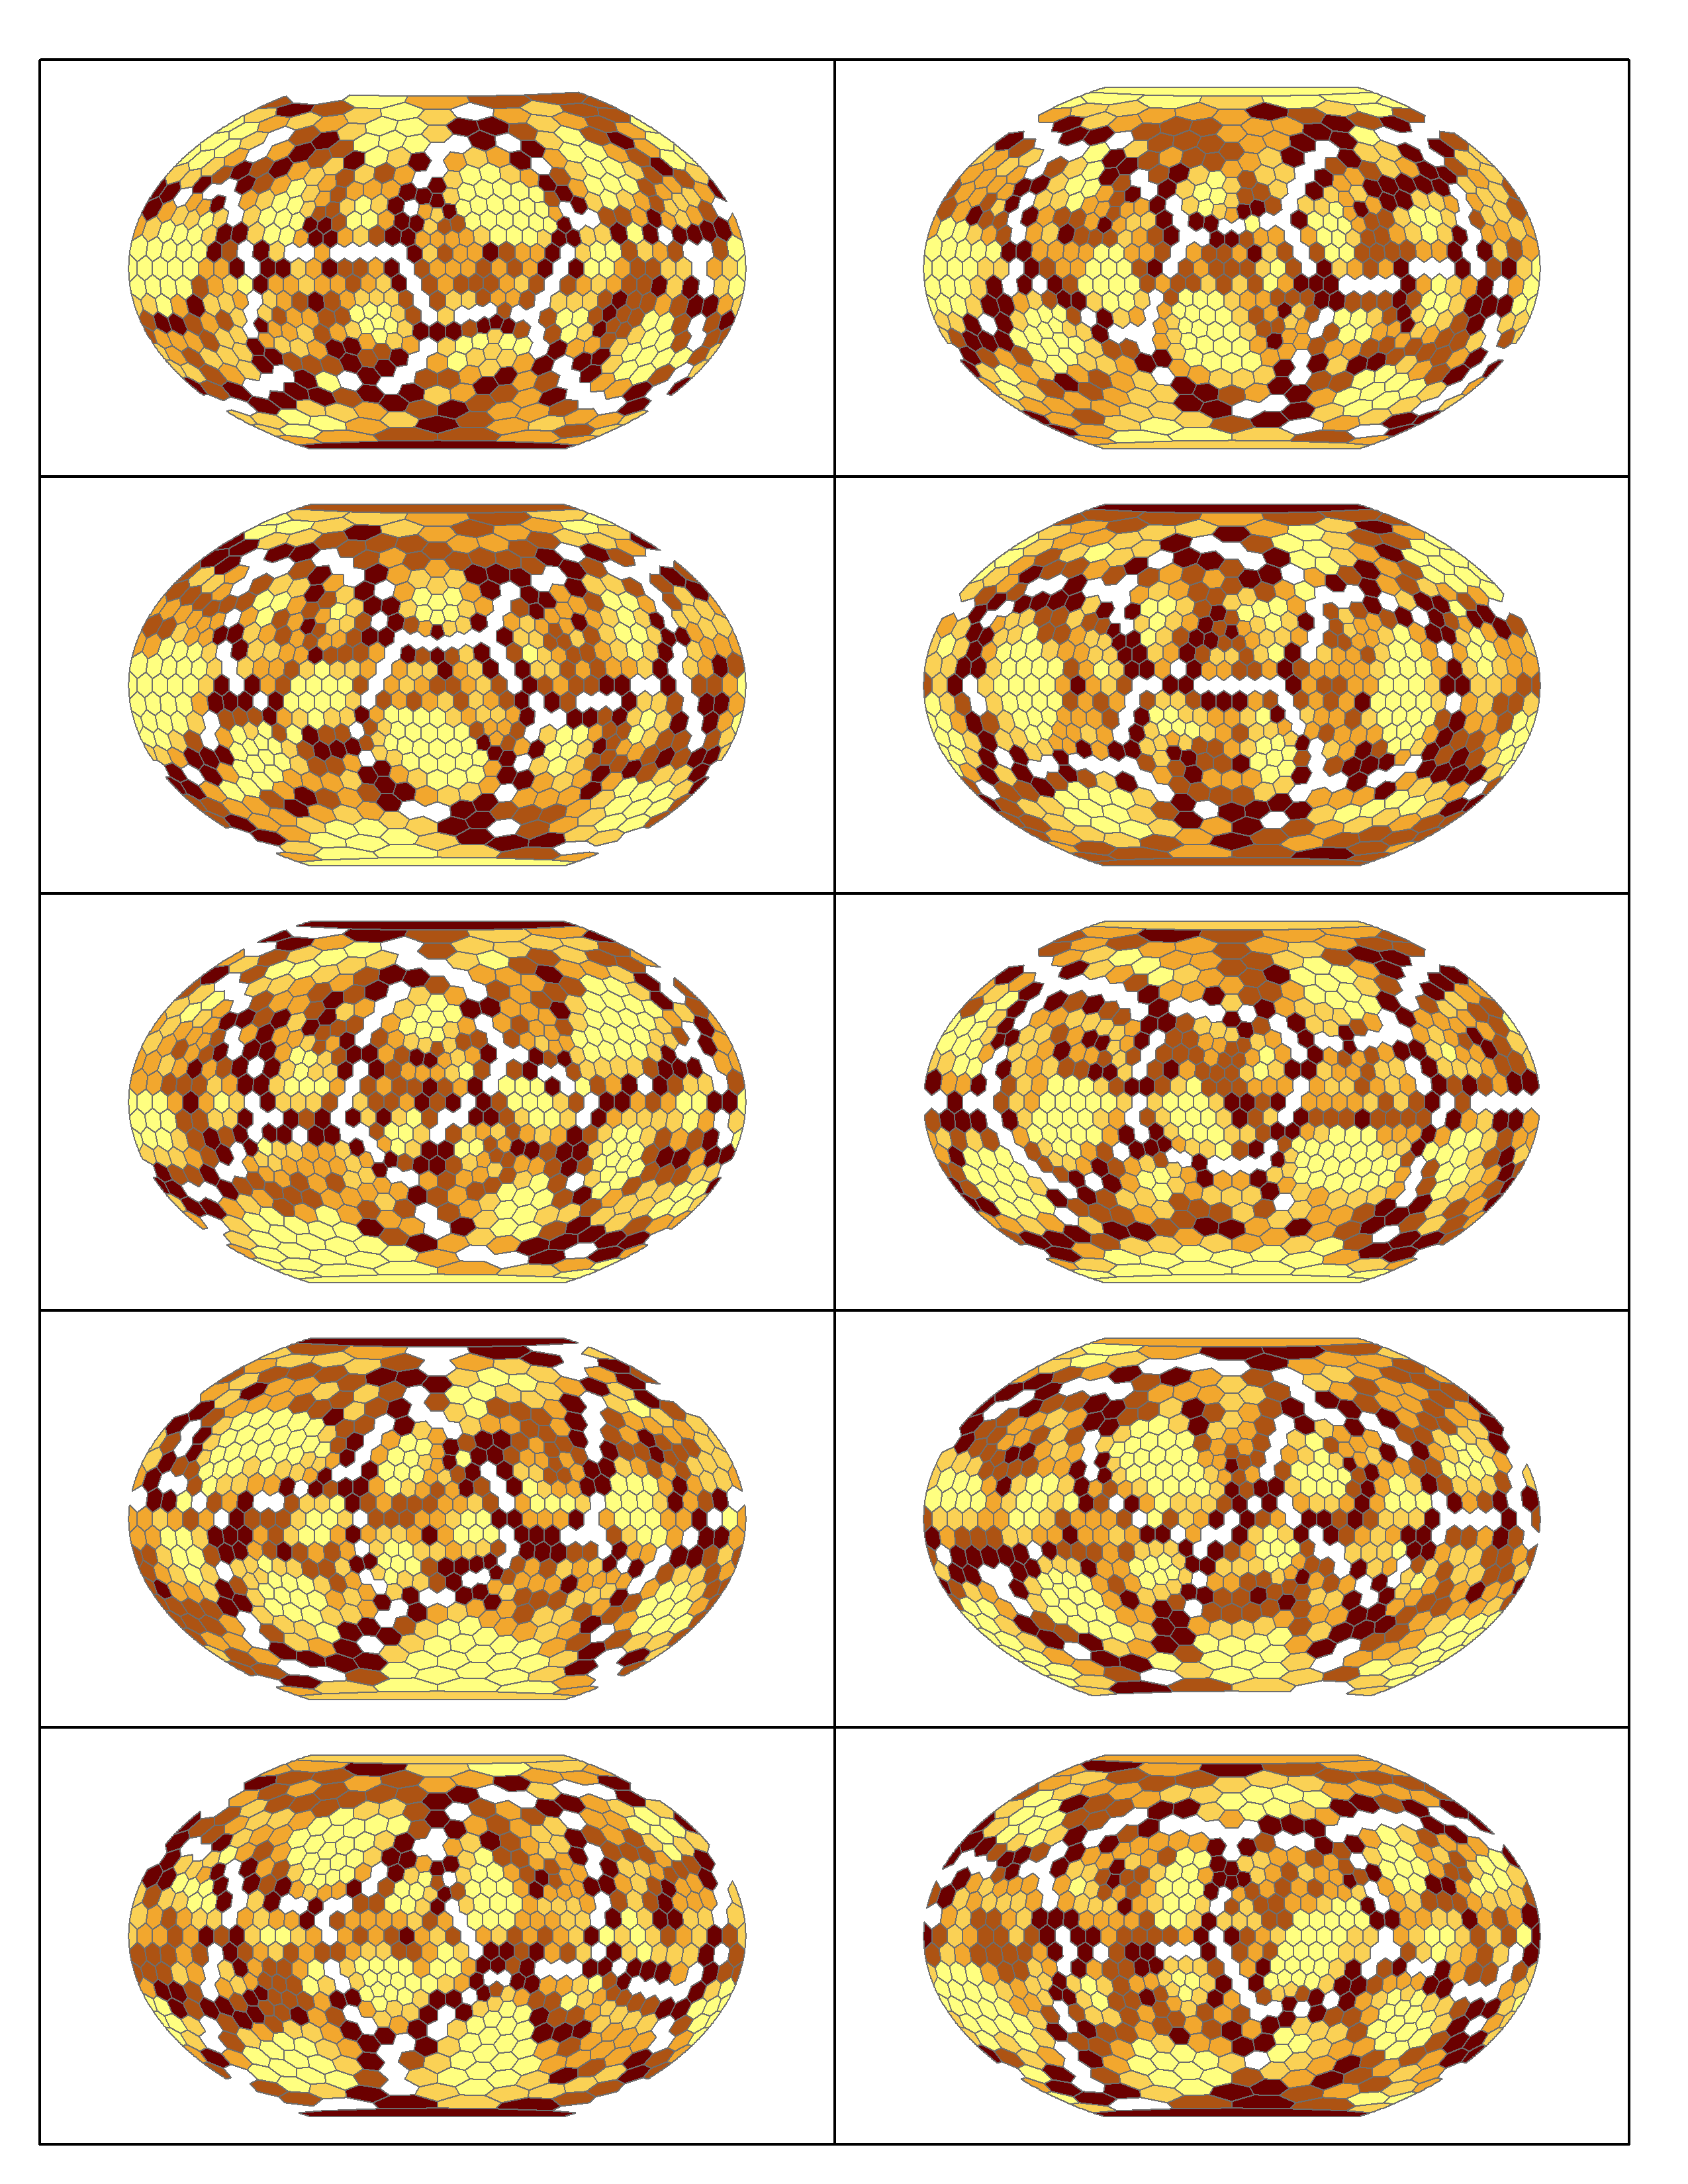
\includegraphics[width=0.5\linewidth]{geodesic_thesis_7c.png}
}
\caption{Internal variance mapping for each of the forty SOMs. Darker colors
represent neurons that display larger internal variance. Neurons for which
an internal variance could not be calculated are not displayed.}
\label{ten}
\end{minipage}
\end{figure}

\begin{figure}
\begin{minipage}{\textwidth}
  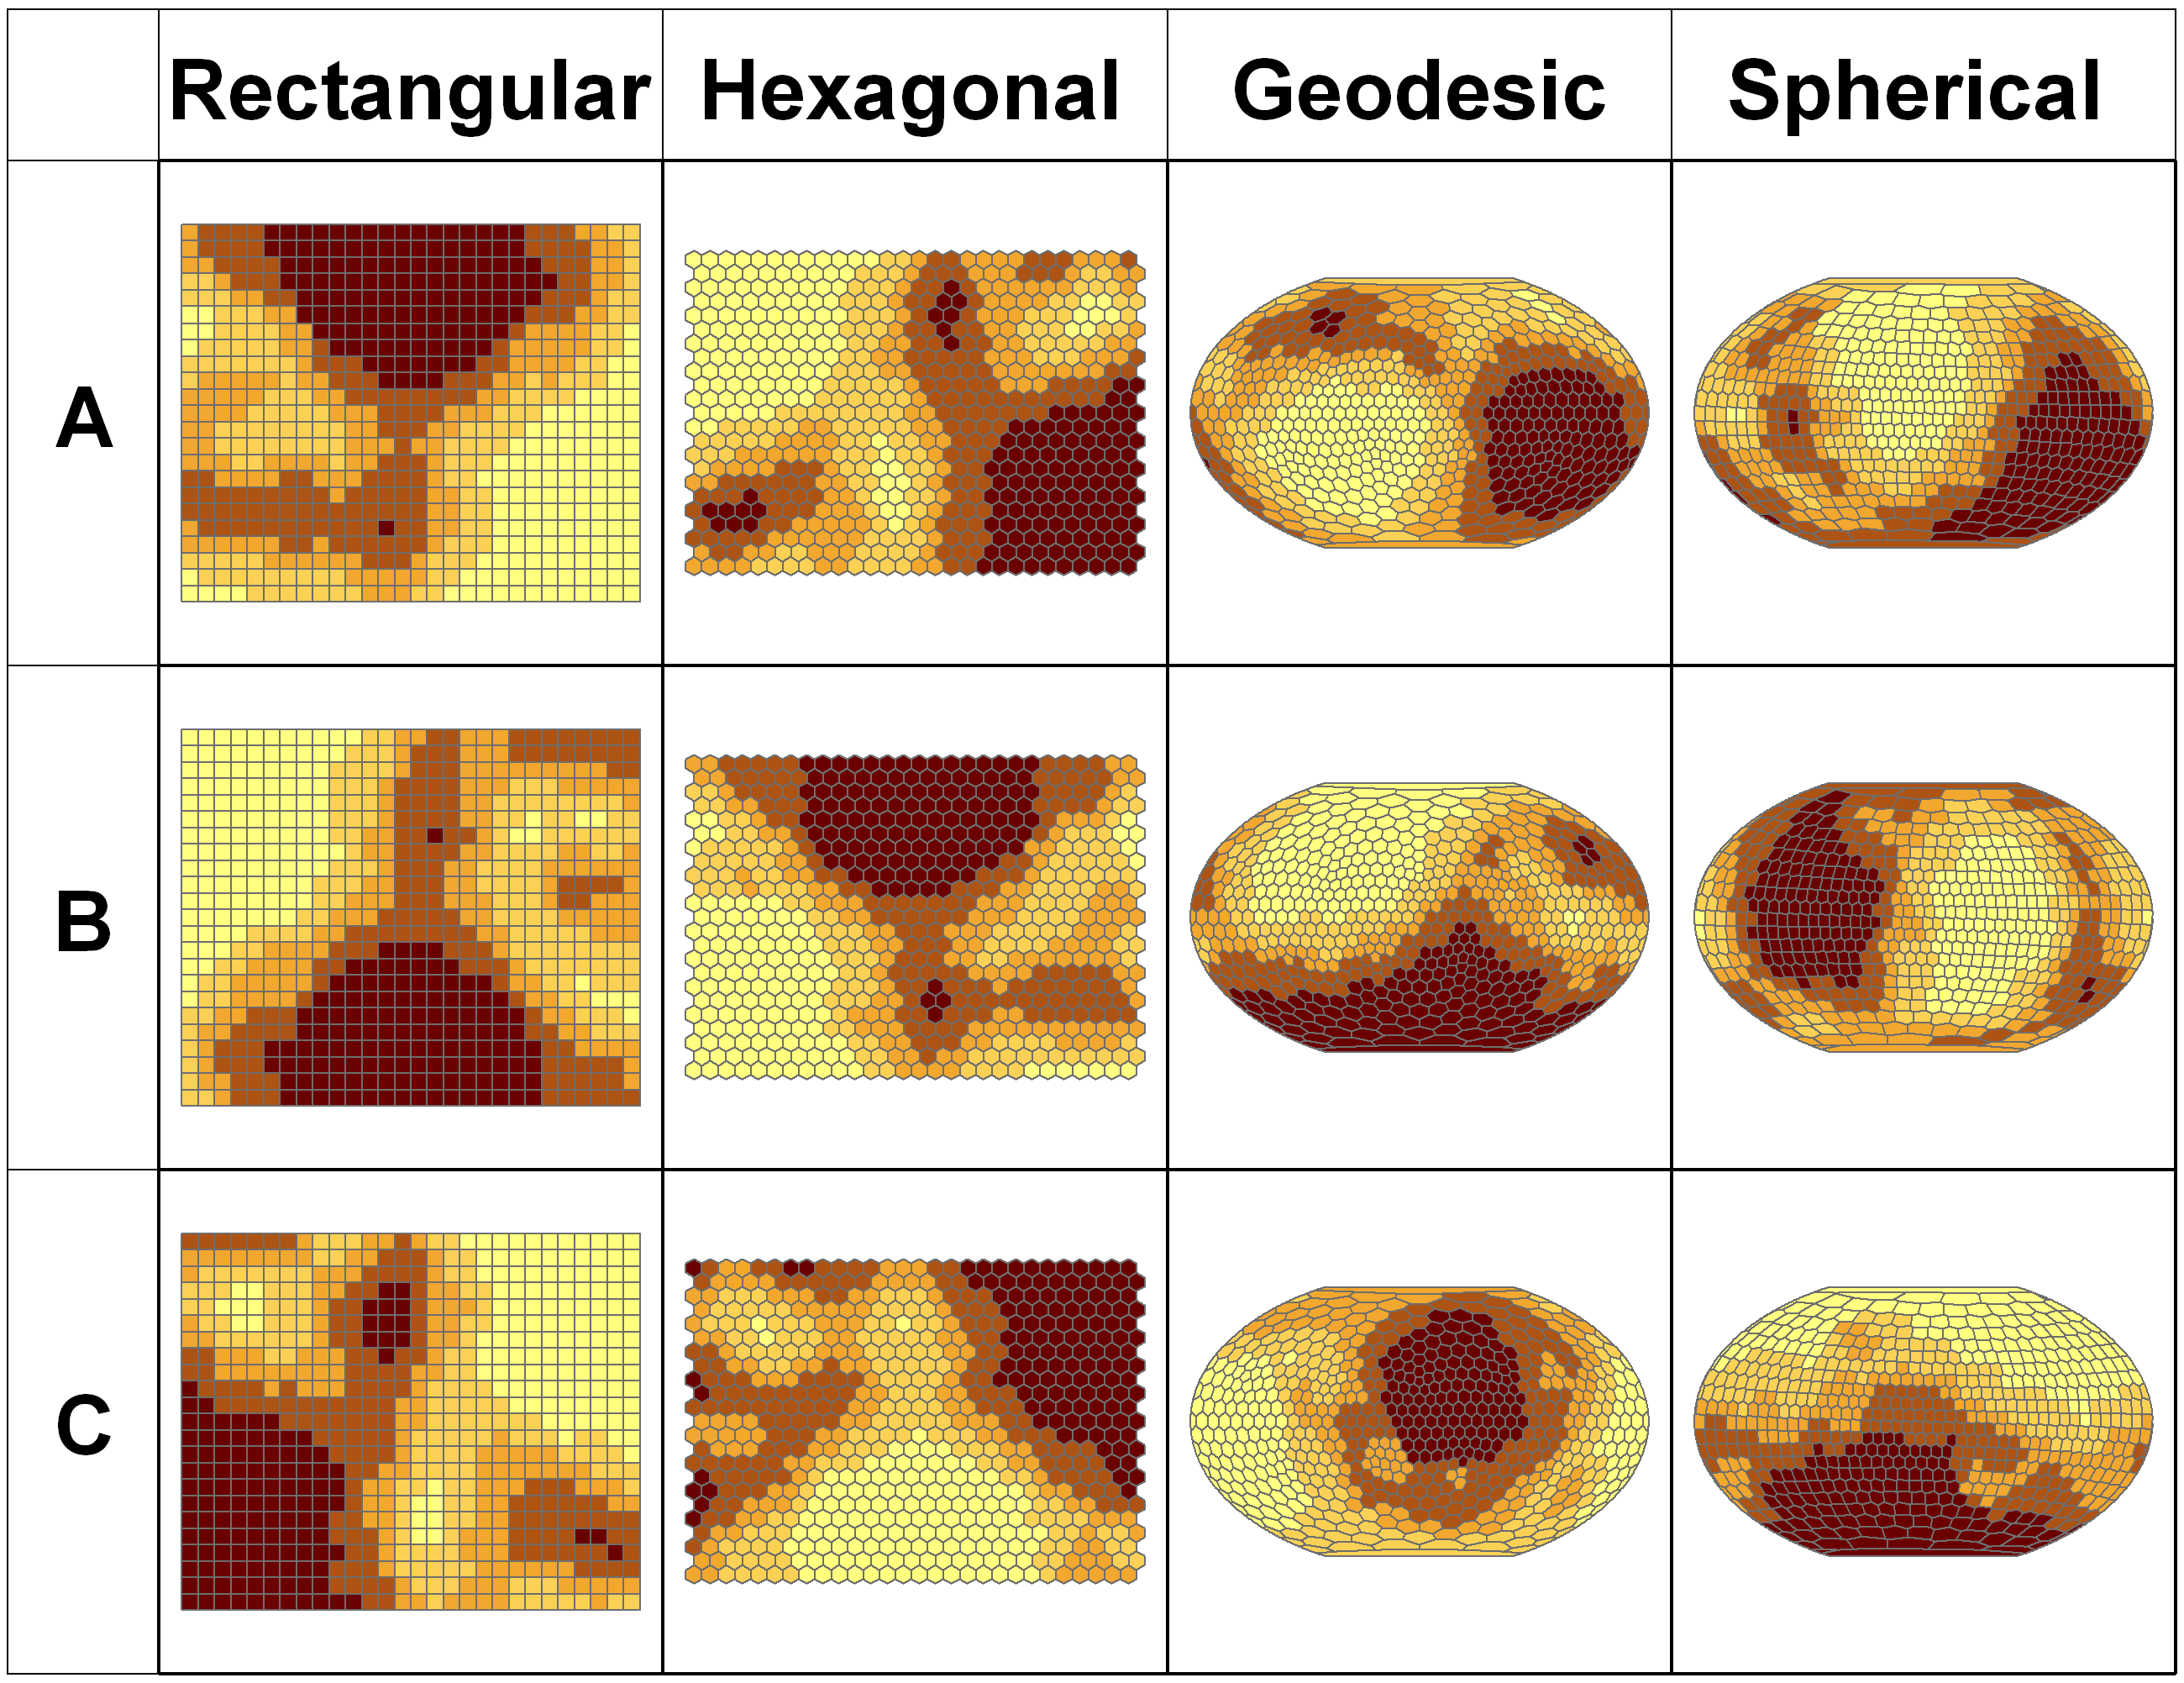
\includegraphics[width=\linewidth]{cplanes.png}
  \caption{The first (A), second (B) and third (C) component planes are shown
for the first simulation of each topology.  These component planes show how
the original dimensions are represented in the trained SOMs.}
  \label{cplanes}
\end{minipage}\end{figure}


\begin{figure}
\centering
\begin{minipage}{\textwidth}
\subfigure[Rectangular Topology]{
  \label{cluster:rook}
  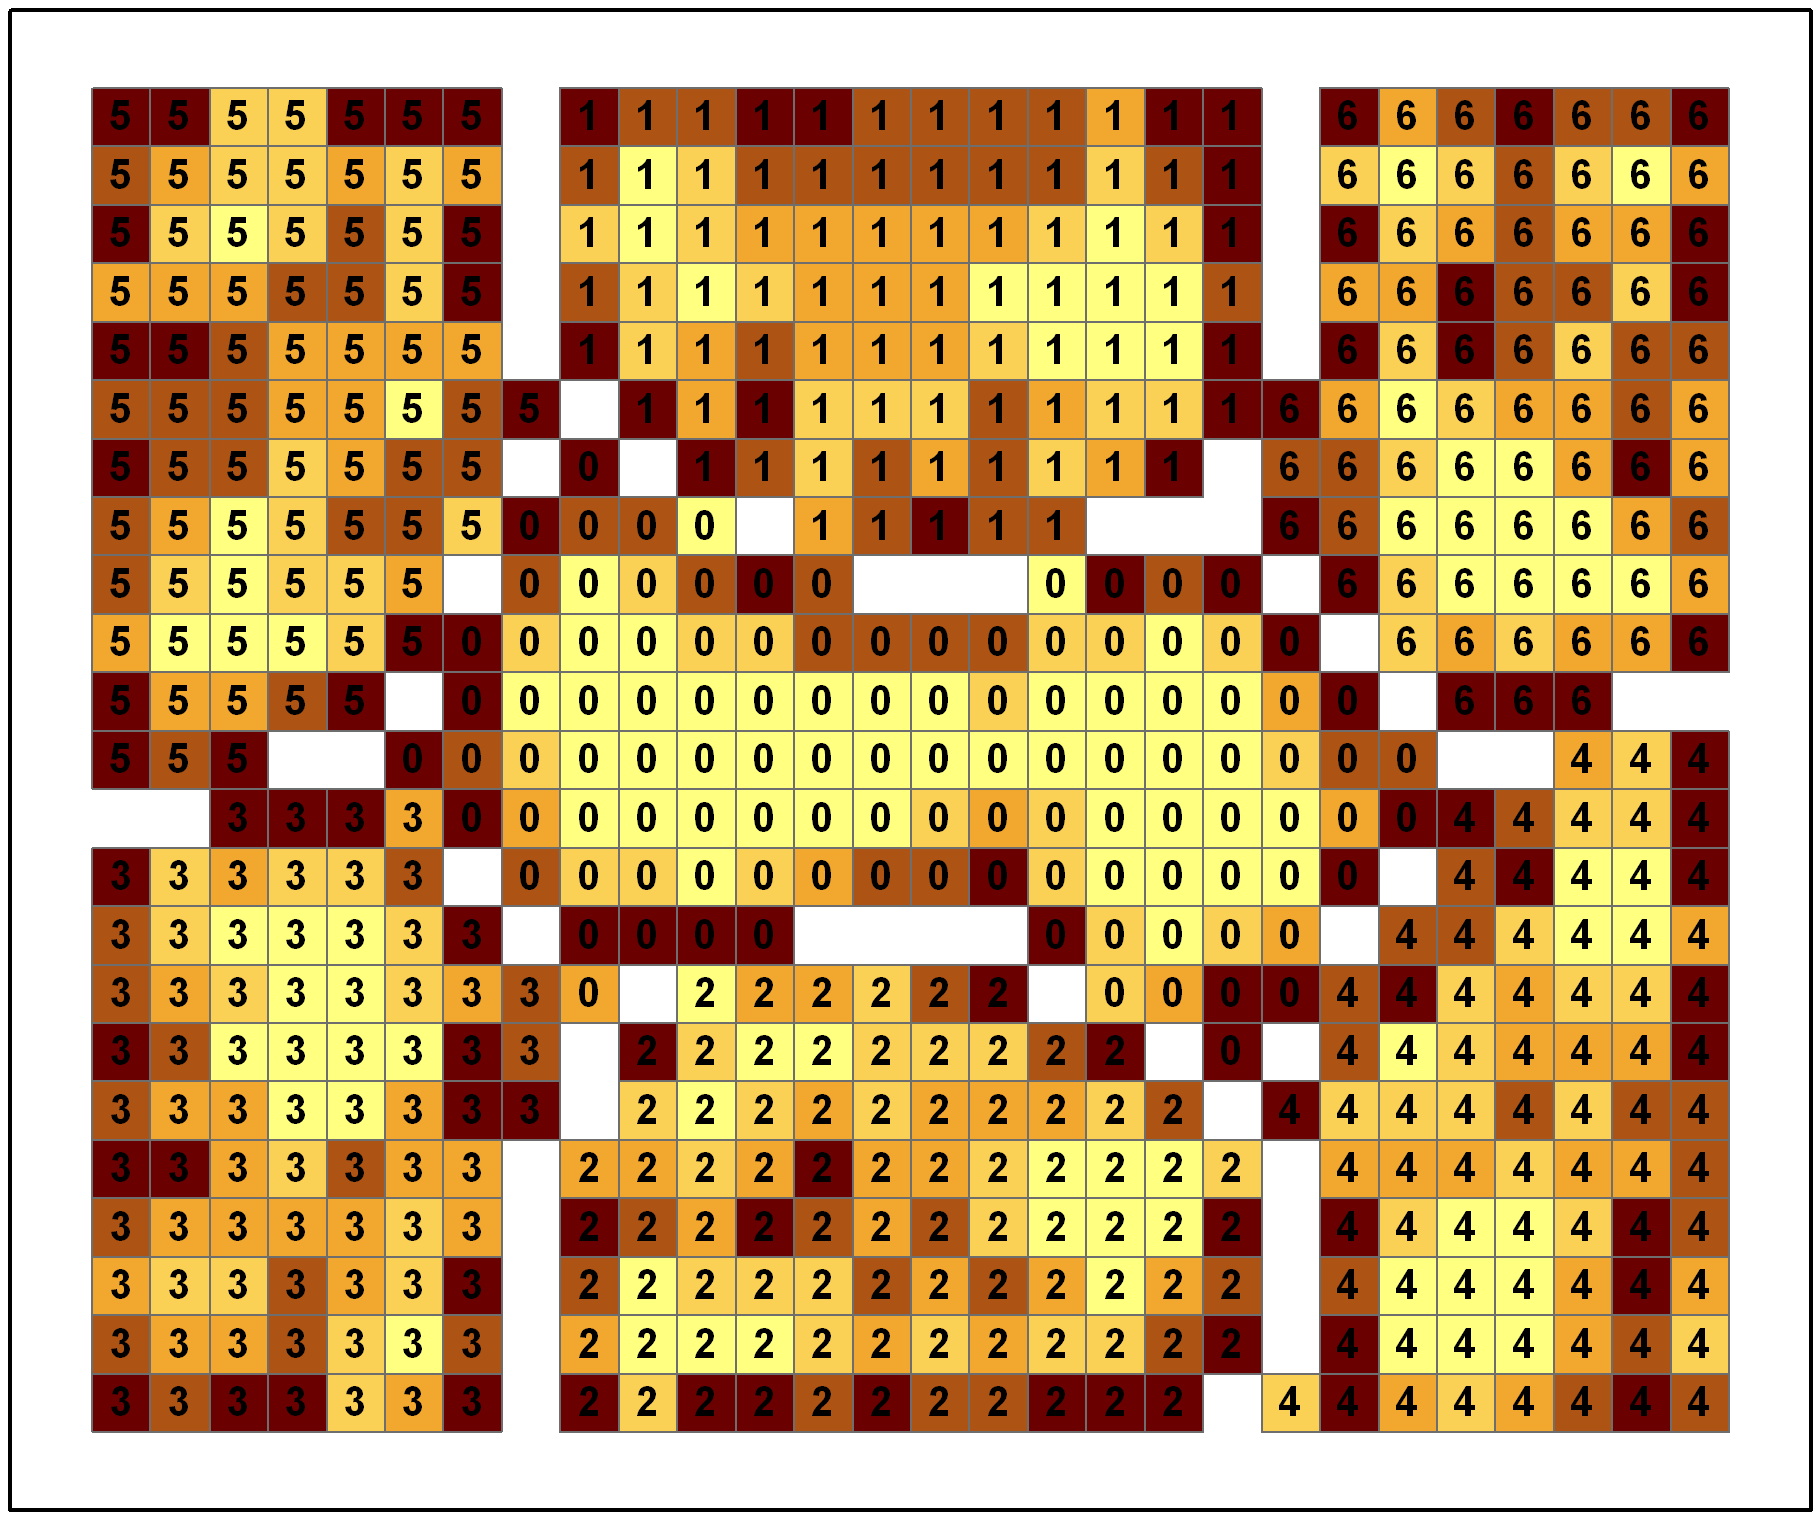
\includegraphics[width=0.5\linewidth]{rook_clusters.png}
}
\subfigure[Hexagonal Topology]{
  \label{cluster:hex}
  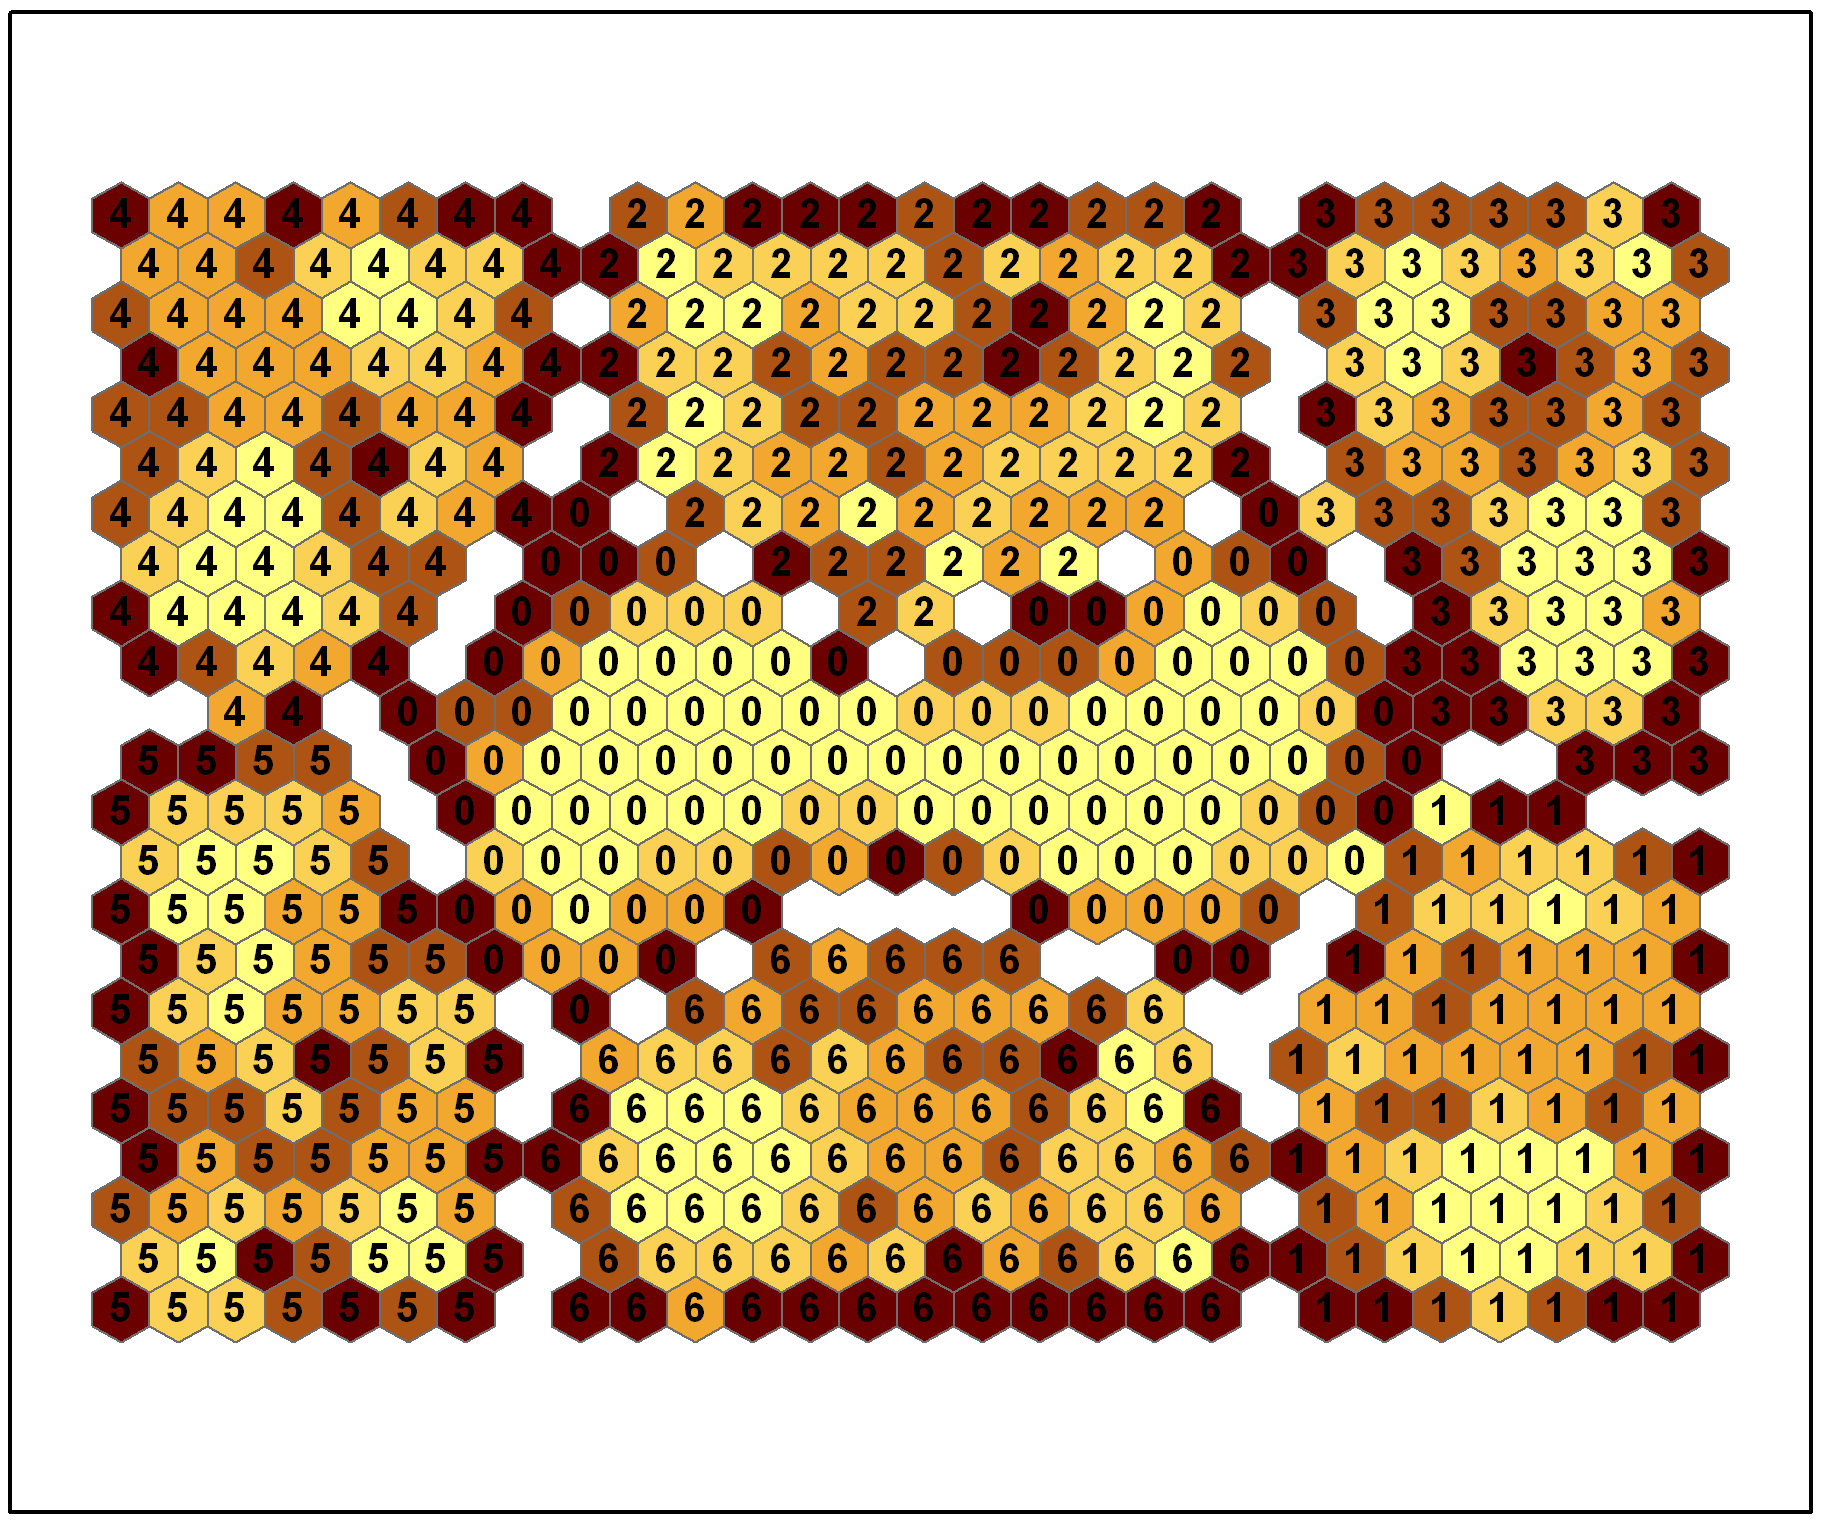
\includegraphics[width=0.5\linewidth]{hex_clusters.png}
}
\subfigure[Spherical Topology]{
  \label{cluster:graph}
  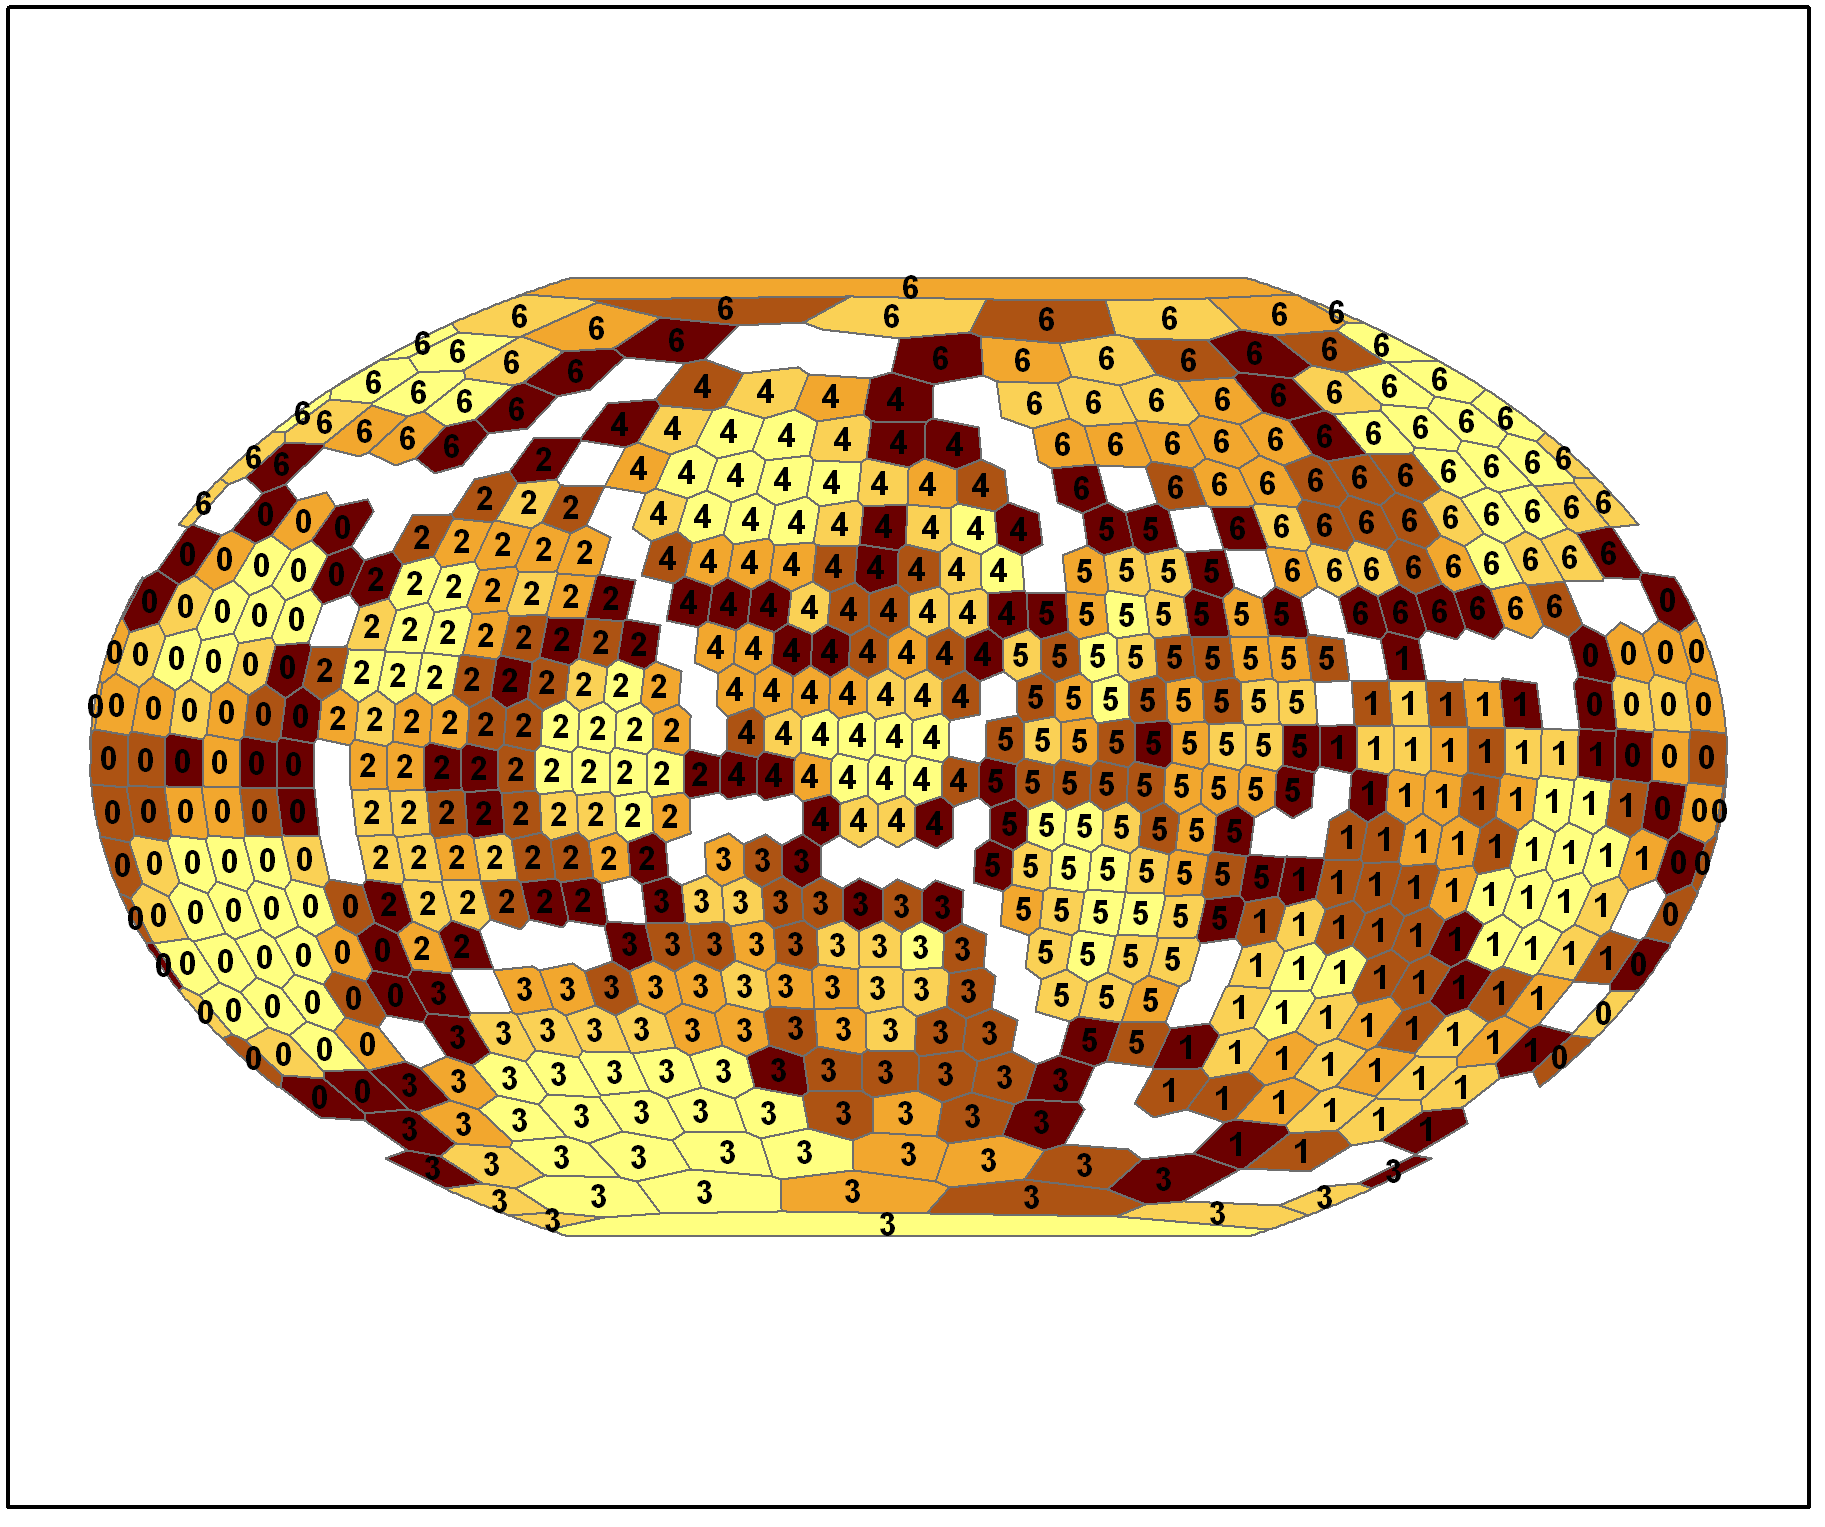
\includegraphics[width=0.5\linewidth]{sphere_clusters.png}
}
\subfigure[Geodesic Sphere Topology]{
  \label{cluster:geodesic}
  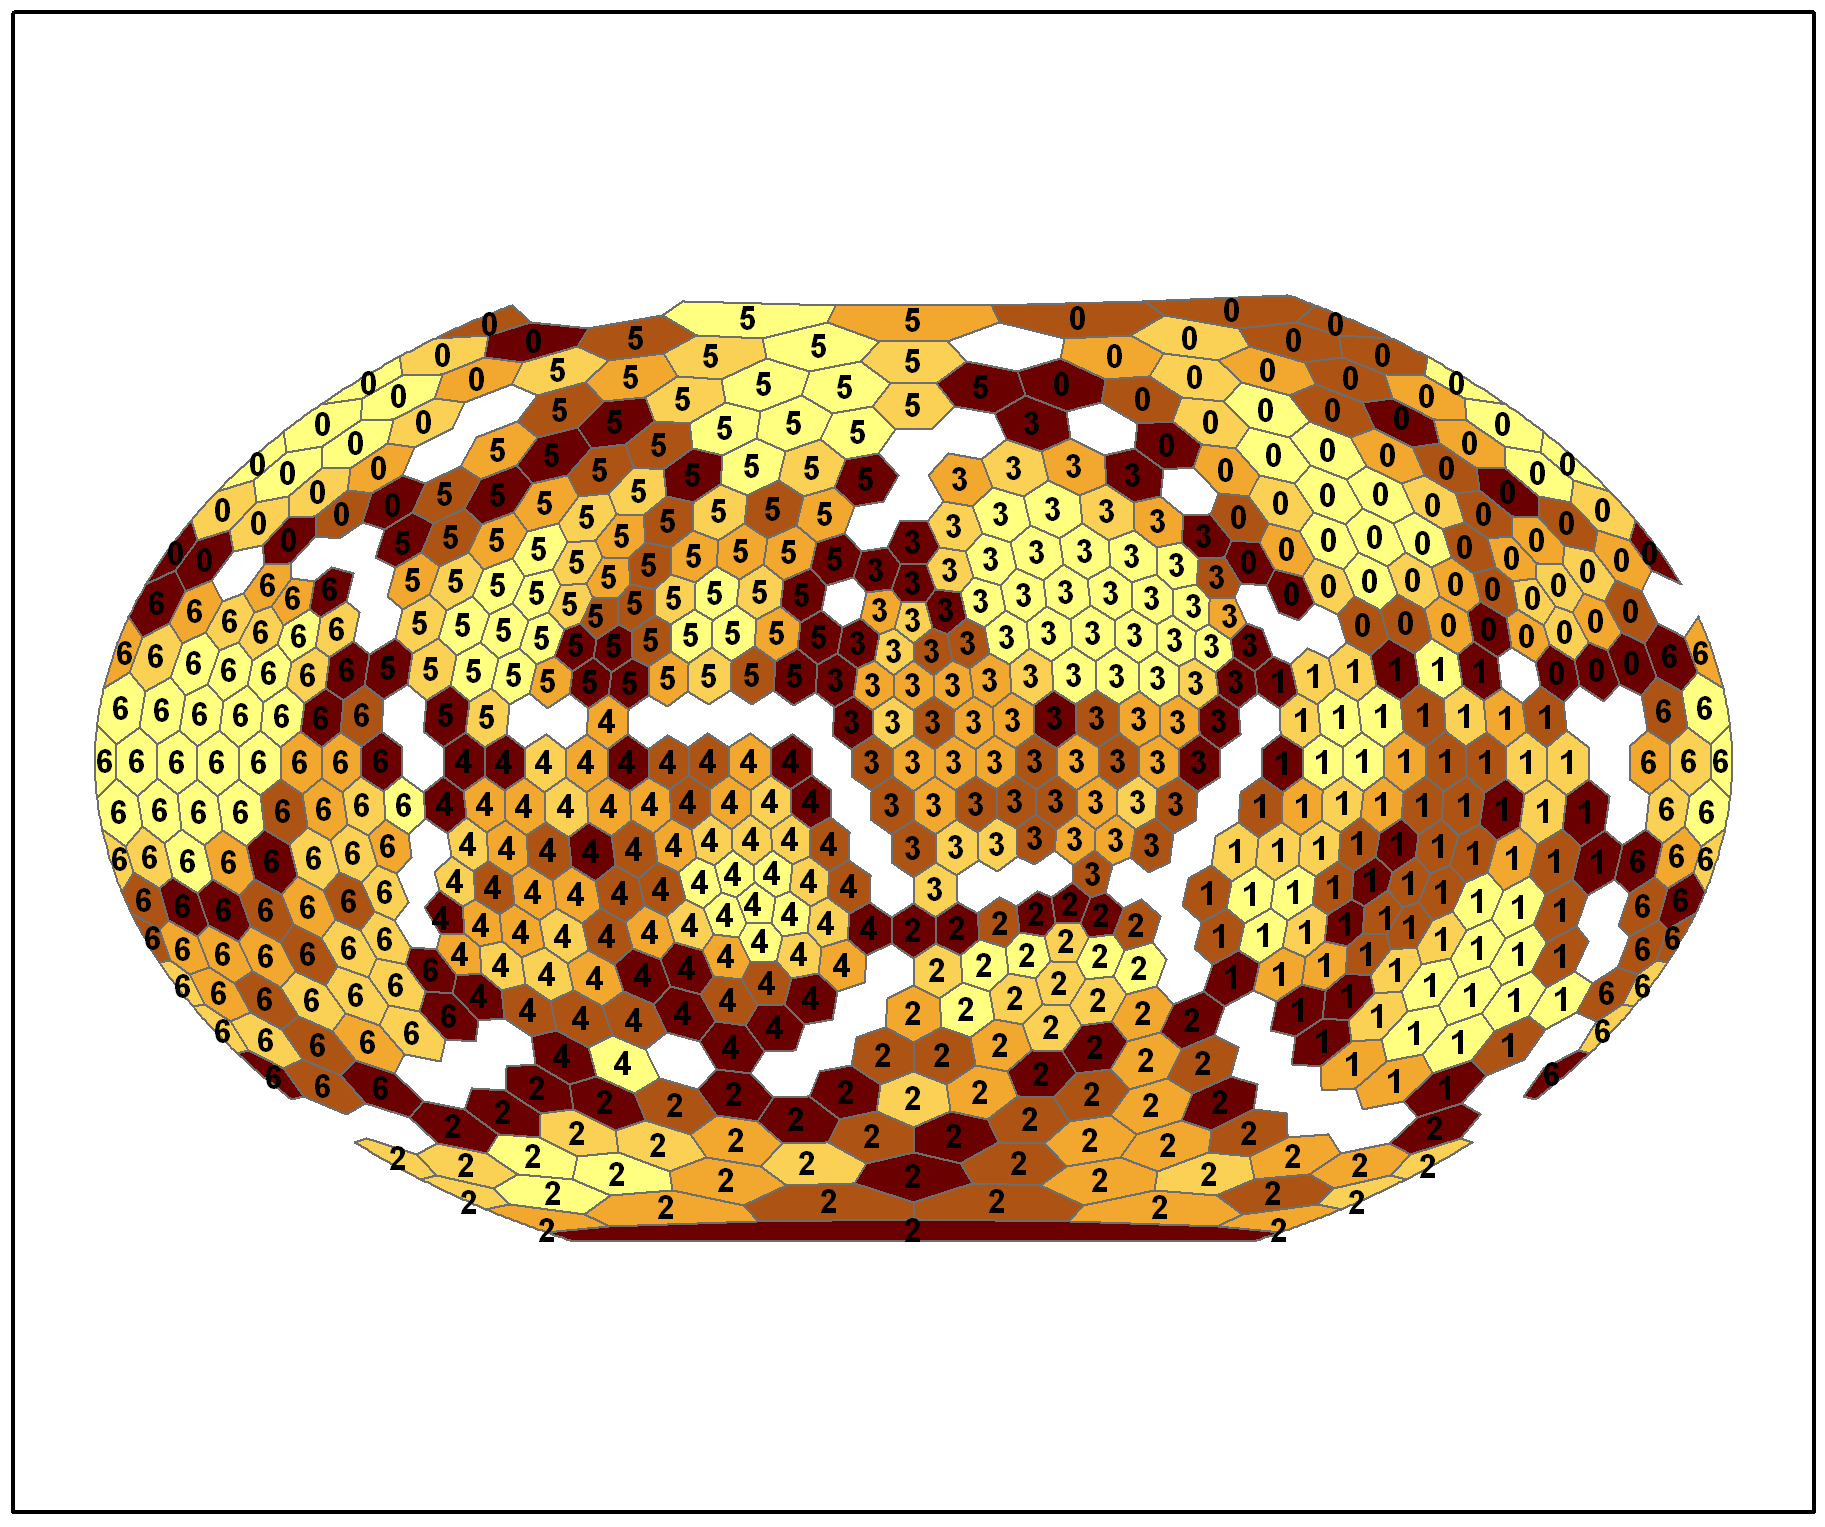
\includegraphics[width=0.5\linewidth]{geodesic_clusters.png}
}
\caption{Detailed internal variance mapping for each topology. Darker colors
represent neurons that display larger internal variance. Neurons for which
an internal variance could not be calculated are not displayed. The numbers
represent primary cluster mapped at that neuron.}
\label{cluster}
\end{minipage}
\end{figure}




